\subsection{Experiment Details}
\label{app:experiment_details}

\subsubsection{Uniform Quantization Review}
A \textit{$b$-bit uniform quantization} $Q_{b,r}(x)$ of a real number $x \in [-r,r]$ is computed as follows:
First, the interval $[-r,r]$ is divided into $2^b - 1$ sub-intervals of equal size.
Then, $x$ is rounded to either the top or bottom of the sub-interval $[\ulx,\olx]$ containing $x$, where $\ulx = r + j\frac{2r}{2^b-1}$ and $\olx = r + (j+1)\frac{2r}{2^b-1}$, for $j\in\{0,1,\ldots,2^b-2\}$.
Given this rounded value, one can simply store the $b$-bit integer $j$ or $j+1$ in place of the real-valued $x$, depending on whether $x$ was rounded to $\ulx$ and $\olx$ respectively.
In this work, we will consider a deterministic rounding scheme which rounds $x$ to the nearest value, and a stochastic rounding scheme which rounds $x$ up or down in such a way that the expected value is equal to $x$.\footnote{
	This stochastic scheme rounds $x$ to $\ulx$ with probability $\frac{\olx-x}{\olx-\ulx}$ and to $\olx$ with probability $\frac{x-\ulx}{\olx-\ulx}$.
}
In particular, our analysis will focus on the stochastic rounding scheme, while our experiments will include results with both schemes.

%Note that we can upper bound the variance of these rounding schemes using the fact that a bounded random variable in an interval of length $c$ has variance at most $c^2/4$;
%using this fact, we can see that the variances of these rounding schemes are at most $\frac{1}{4} \cdot \Big(\frac{2r}{(2^b-1)}\Big)^2 = \frac{4r^2}{(2^b-1)^2}$.


We are now ready to present the uniform quantization compression algorithm, which we express in pseudo-code in Algorithm~\ref{alg:smallfry}.
The input to the algorithm is an embedding matrix $X \in \RR^{n\times d}$, where $n$ is the size of the vocabulary, and $d$ is the dimension of the embeddings.
We define the function $\clip_r(x) = \max(\min(x,r),-r)$ for any non-negative $r$; when matrices are passed in as inputs to this function, it clips the entries in an element-wise fashion.
The first step in our algorithm is to find the value of $r \in [0,\max(|X|)]$ which minimizes the reconstruction error of the quantized embeddings after $X$ is clipped to $[-r,r]$.
More formally, we let $r^* \defeq \argmin_{r \in [0,\max(|X|)} \|Q_{b,r}(\clip_r(X))-X\|_F$.
We then use this value $r^*$ to clip $X$, and then quantize the clipped embeddings to $b$ bits per entry.

In our experiments, we find $r^*$ to within a specified tolerance $\eps > 0$ using the golden-section search algorithm \citep{golden53}.
To avoid stochasticity impacting the search process, we always use deterministic rounding in the search for $r^*$, even if we use stochastic quantization in the final quantization.
%this choice also allows us to more cleanly compare deterministic vs.\ stochastic rounding, since they will always use the same value of $r^*$.


\subsubsection{Empirical Comparison of Compression Methods}

\subsubsection{Dimension vs. Precision Trade-off}

\subsection{Extended Results}
\label{app:experiment_results}
In Figure~\ref{fig:all_sentiment} we present all our sentiment analysis results, for our different embedding types and the different sentiment analysis datasets.
%\todo{I commented out large figure}
%\begin{figure}
%	\centering
%	\begin{tabular} {c c c}
%	% MPQA
%	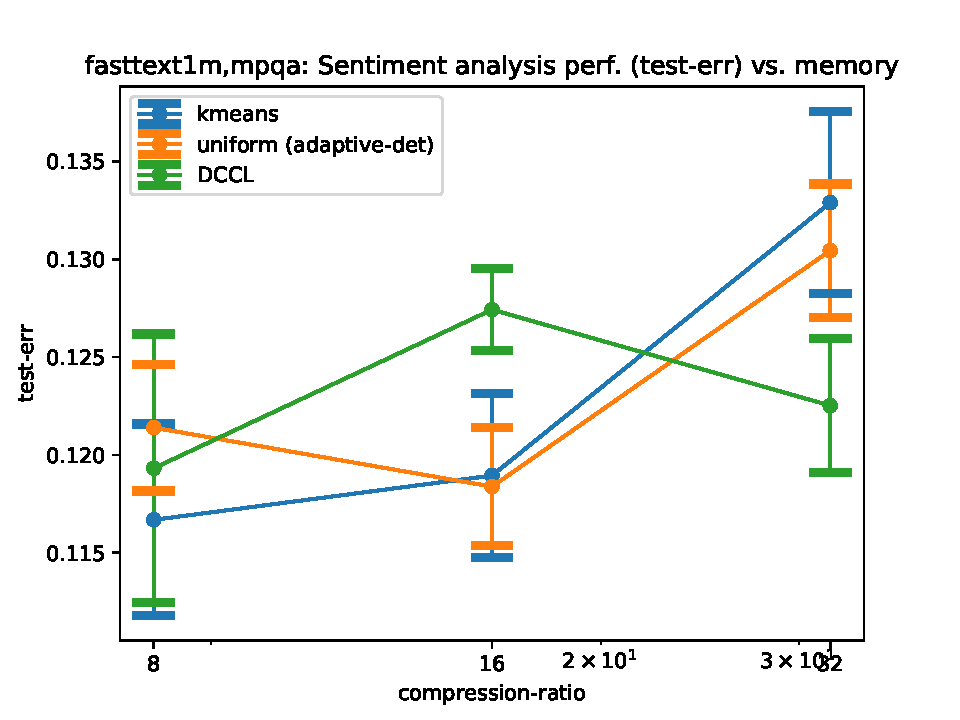
\includegraphics[width=0.28\linewidth]{figures/fasttext1m_mpqa_test-err_vs_compression.pdf} &
%	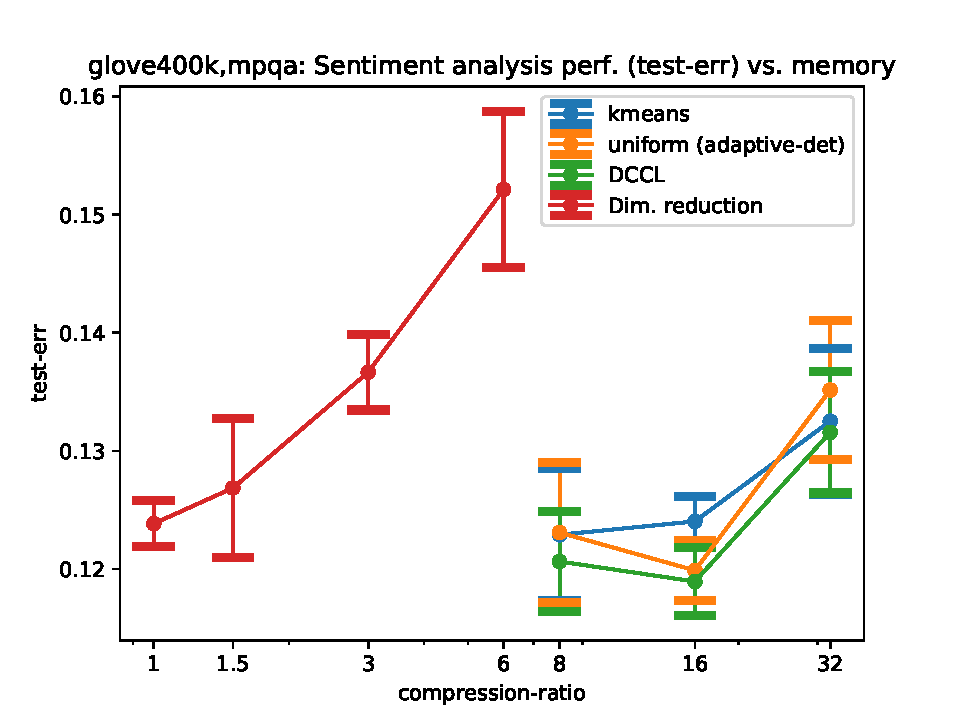
\includegraphics[width=0.28\linewidth]{figures/glove400k_mpqa_test-err_vs_compression.pdf} &
%	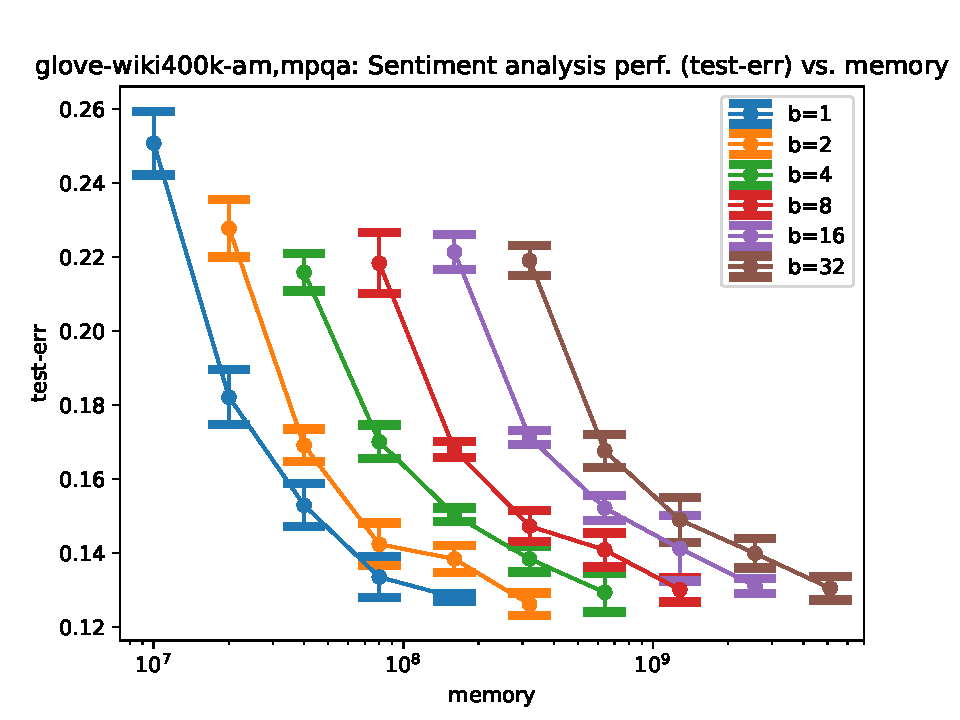
\includegraphics[width=0.28\linewidth]{figures/glove-wiki400k-am_mpqa_test-err_vs_compression.pdf} \\[-0.5em]
%	% TREC
%	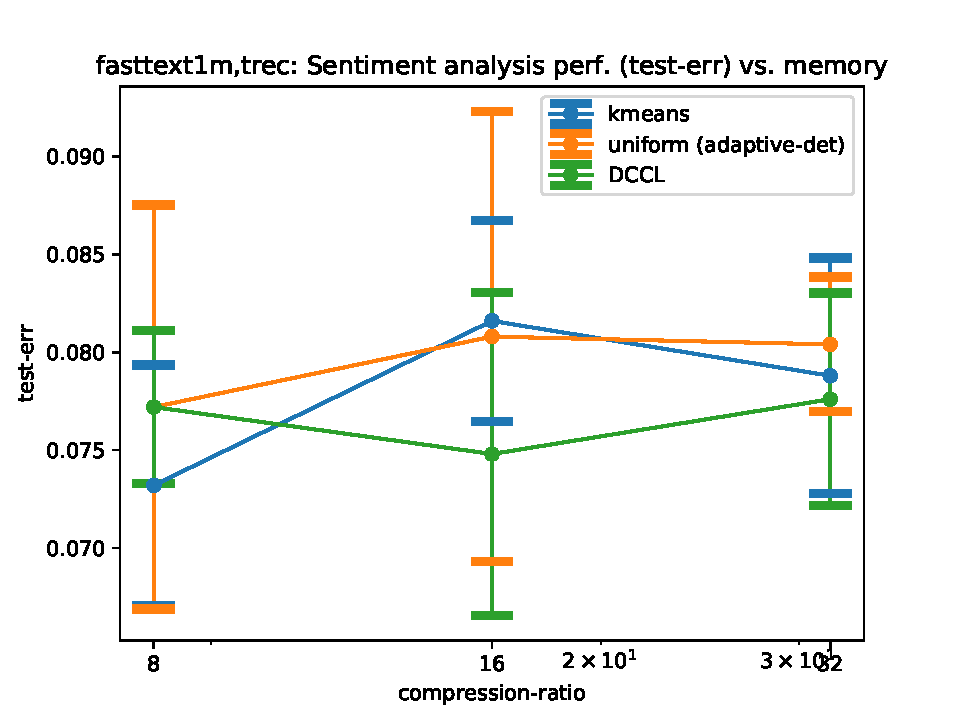
\includegraphics[width=0.28\linewidth]{figures/fasttext1m_trec_test-err_vs_compression.pdf} &
%	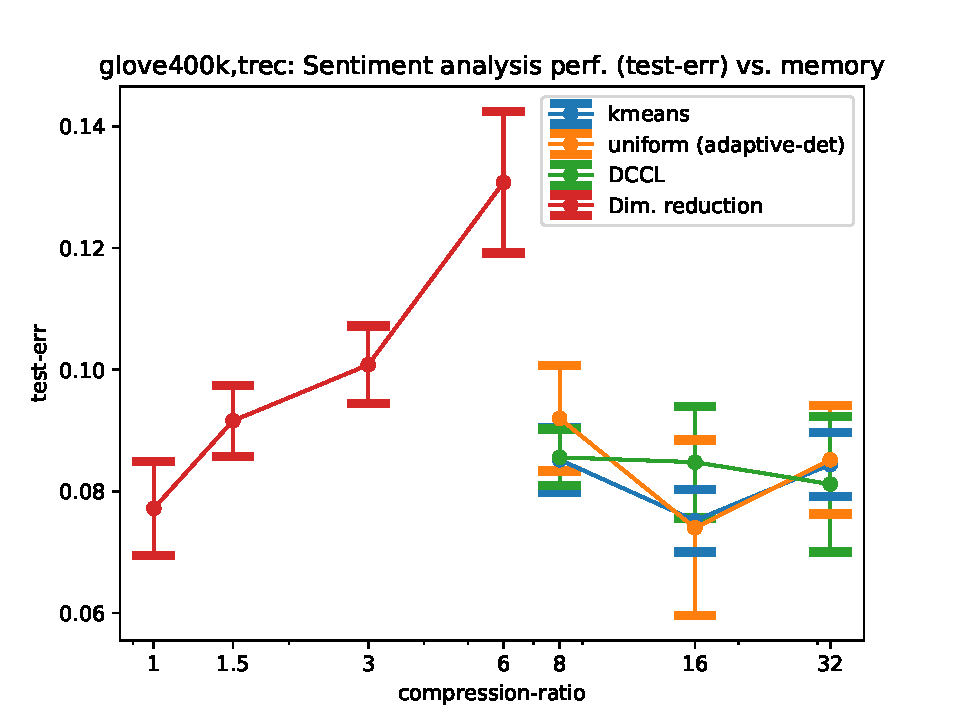
\includegraphics[width=0.28\linewidth]{figures/glove400k_trec_test-err_vs_compression.pdf} &
%	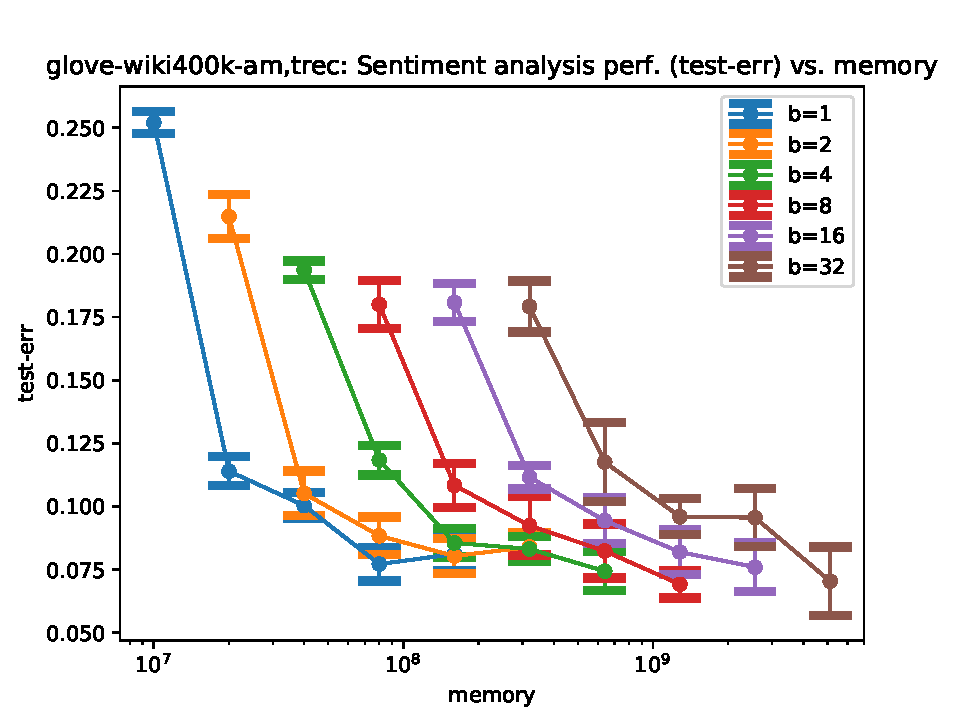
\includegraphics[width=0.28\linewidth]{figures/glove-wiki400k-am_trec_test-err_vs_compression.pdf} \\[-0.5em]
%	% SST
%	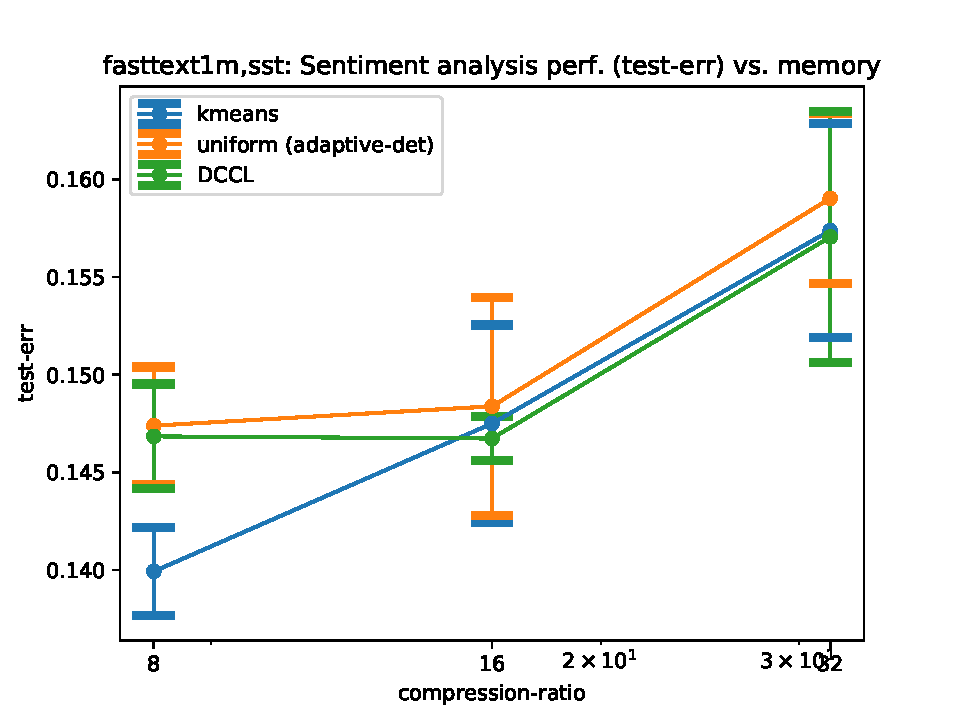
\includegraphics[width=0.28\linewidth]{figures/fasttext1m_sst_test-err_vs_compression.pdf} &
%	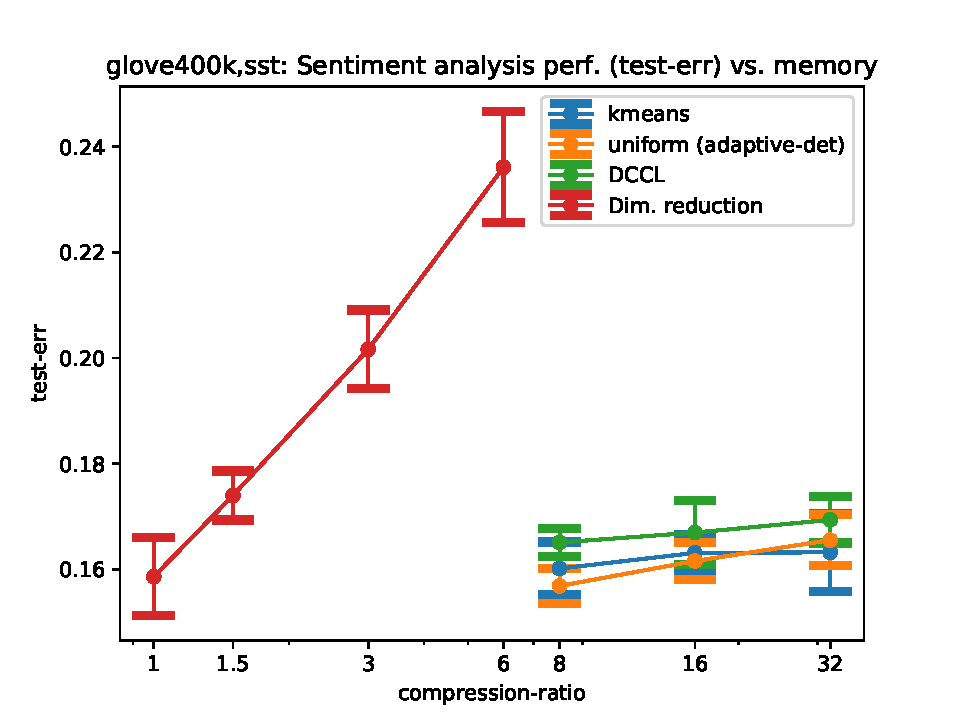
\includegraphics[width=0.28\linewidth]{figures/glove400k_sst_test-err_vs_compression.pdf} &
%	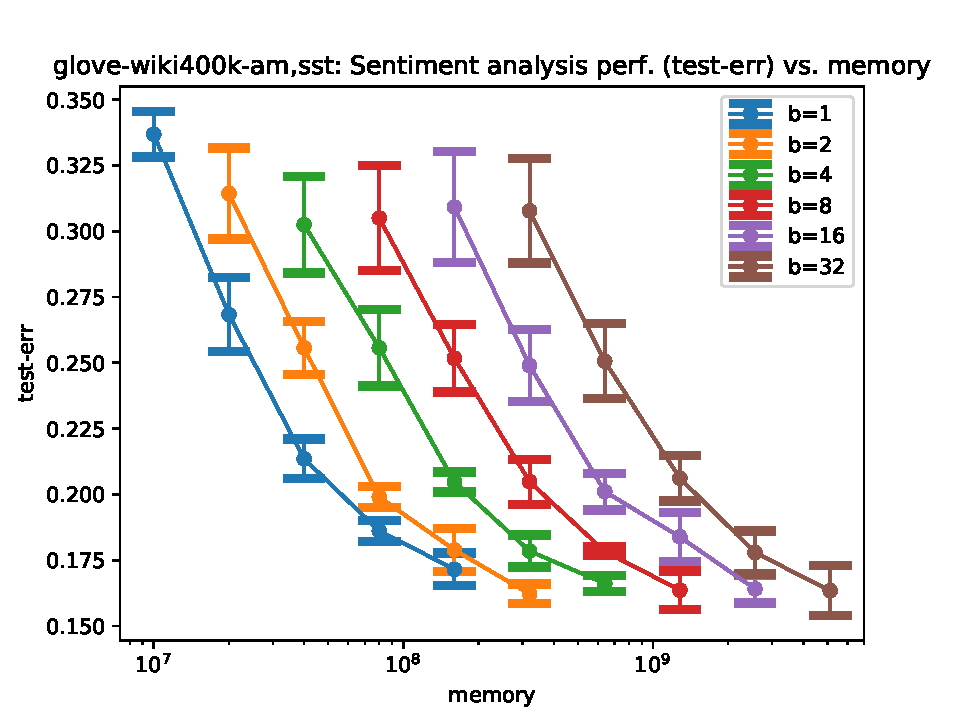
\includegraphics[width=0.28\linewidth]{figures/glove-wiki400k-am_sst_test-err_vs_compression.pdf} \\[-0.5em]
%	% CR
%	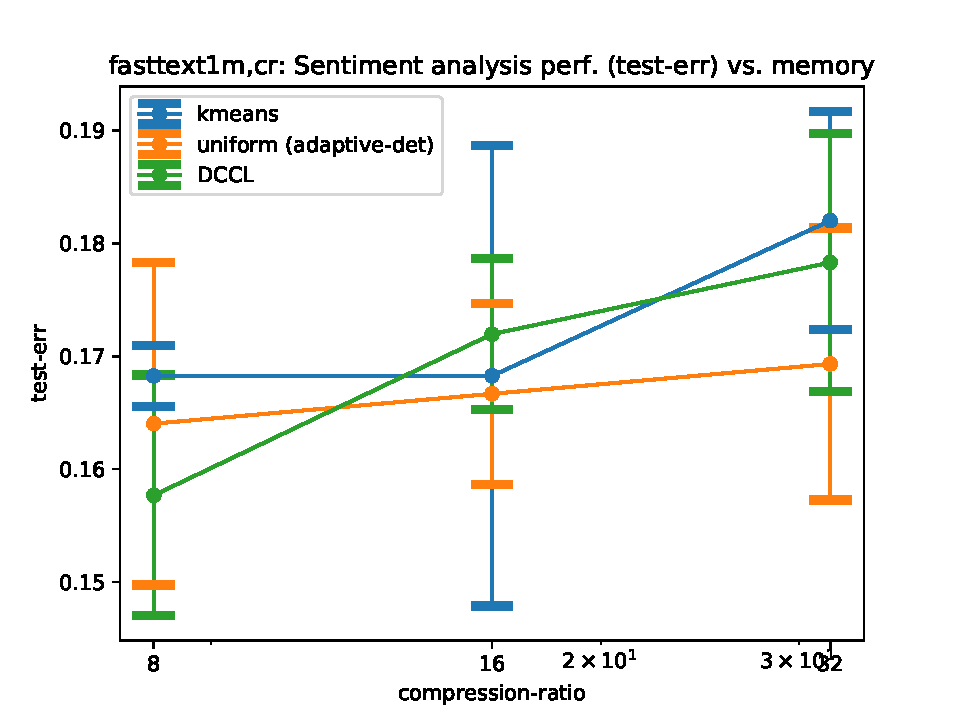
\includegraphics[width=0.28\linewidth]{figures/fasttext1m_cr_test-err_vs_compression.pdf} &
%	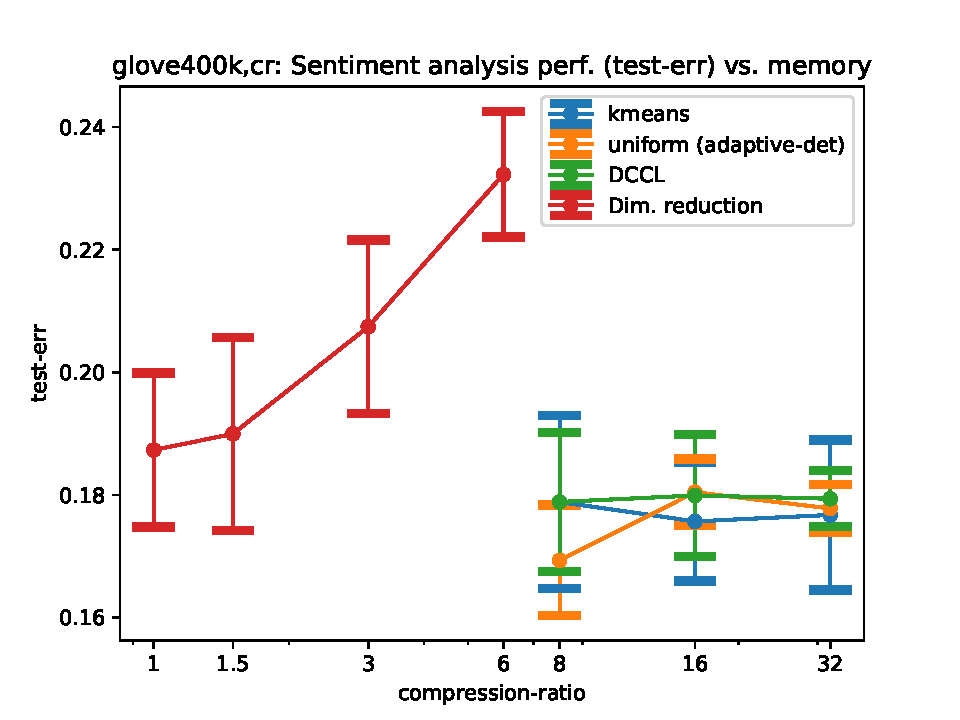
\includegraphics[width=0.28\linewidth]{figures/glove400k_cr_test-err_vs_compression.pdf} &
%	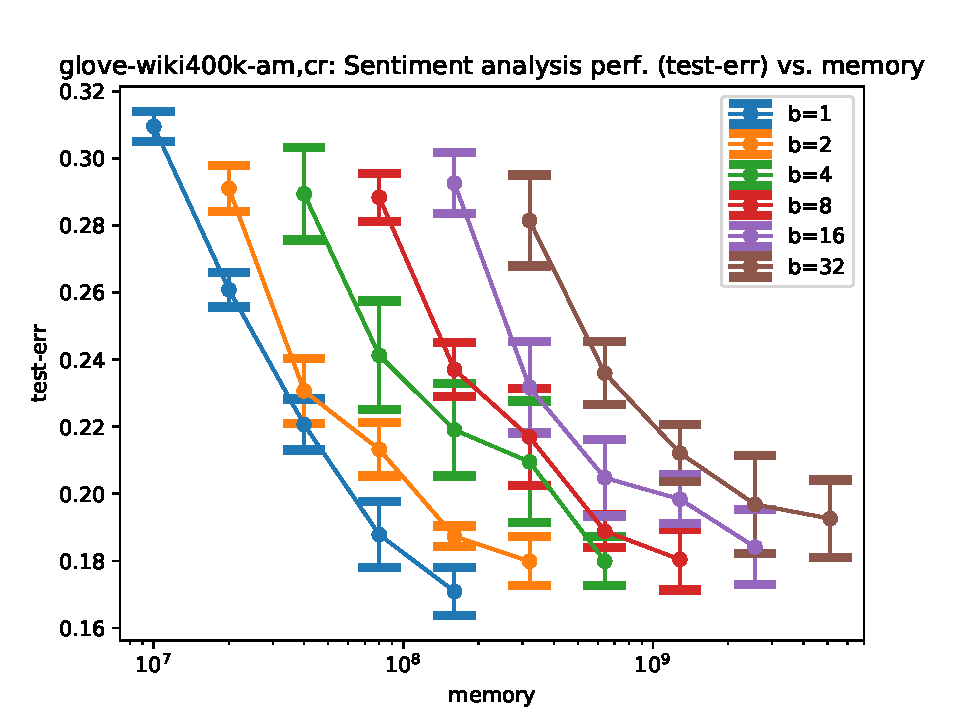
\includegraphics[width=0.28\linewidth]{figures/glove-wiki400k-am_cr_test-err_vs_compression.pdf} \\[-0.5em]
%	% SUBJ
%	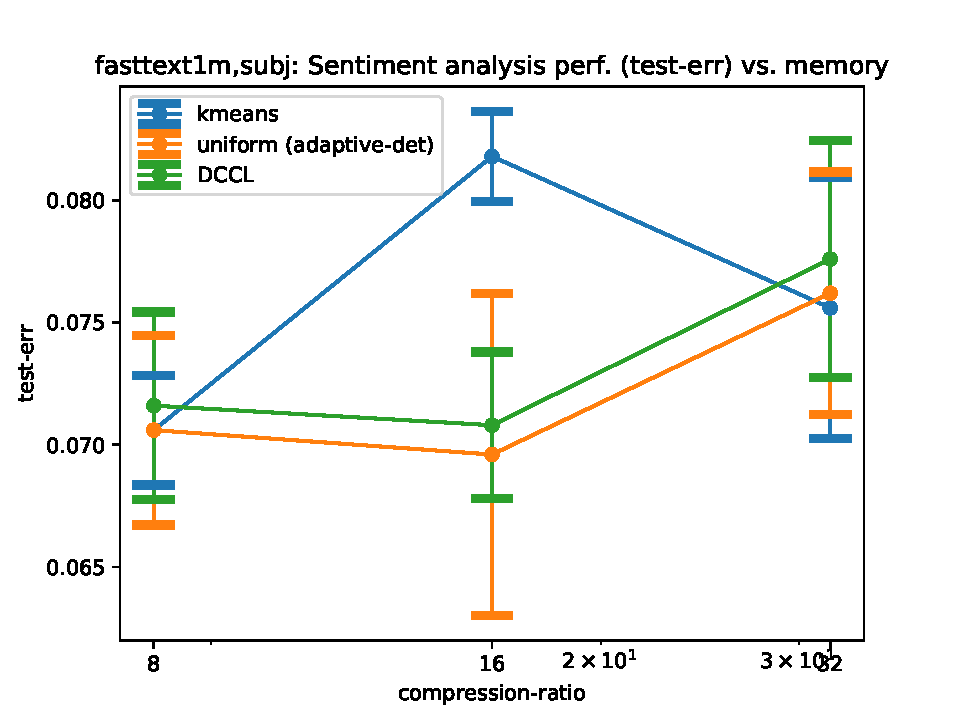
\includegraphics[width=0.28\linewidth]{figures/fasttext1m_subj_test-err_vs_compression.pdf} &
%	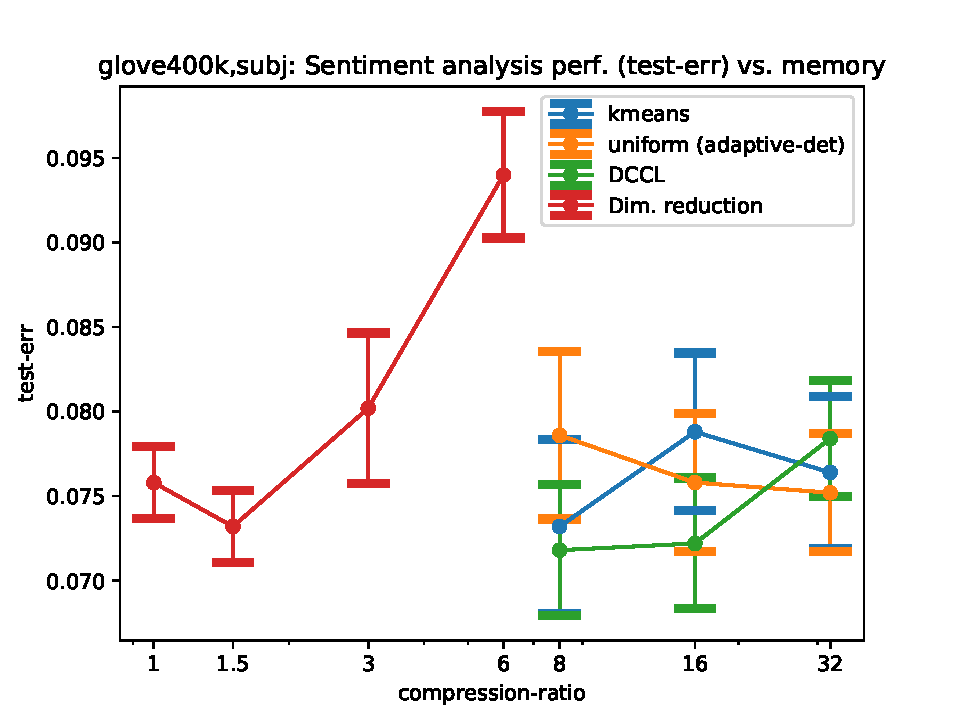
\includegraphics[width=0.28\linewidth]{figures/glove400k_subj_test-err_vs_compression.pdf} &
%	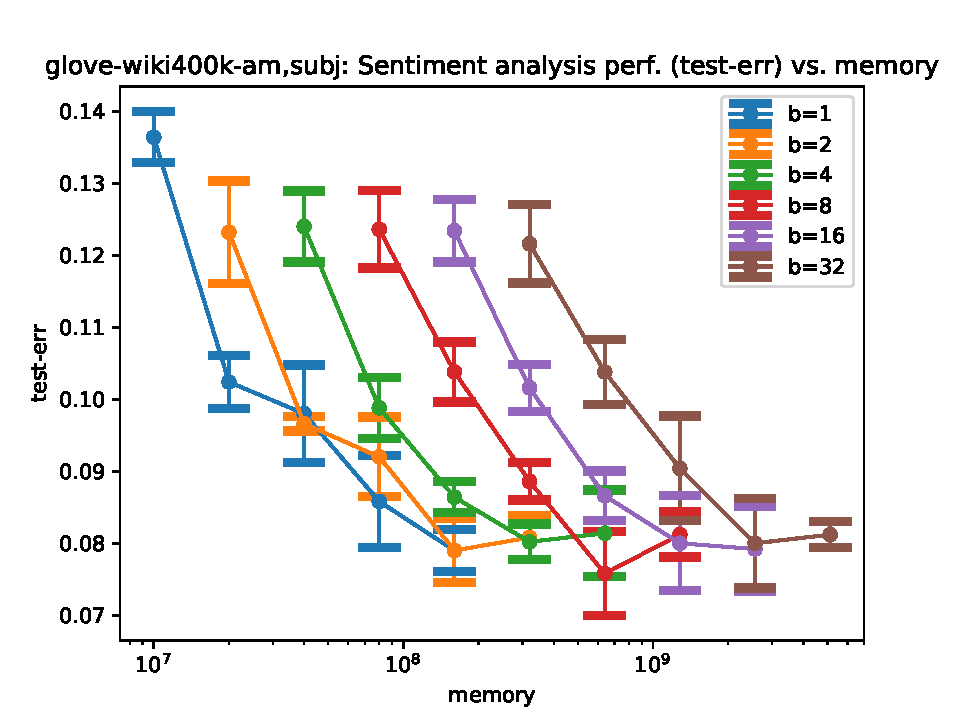
\includegraphics[width=0.28\linewidth]{figures/glove-wiki400k-am_subj_test-err_vs_compression.pdf} \\[-0.5em]
%	% MR
%	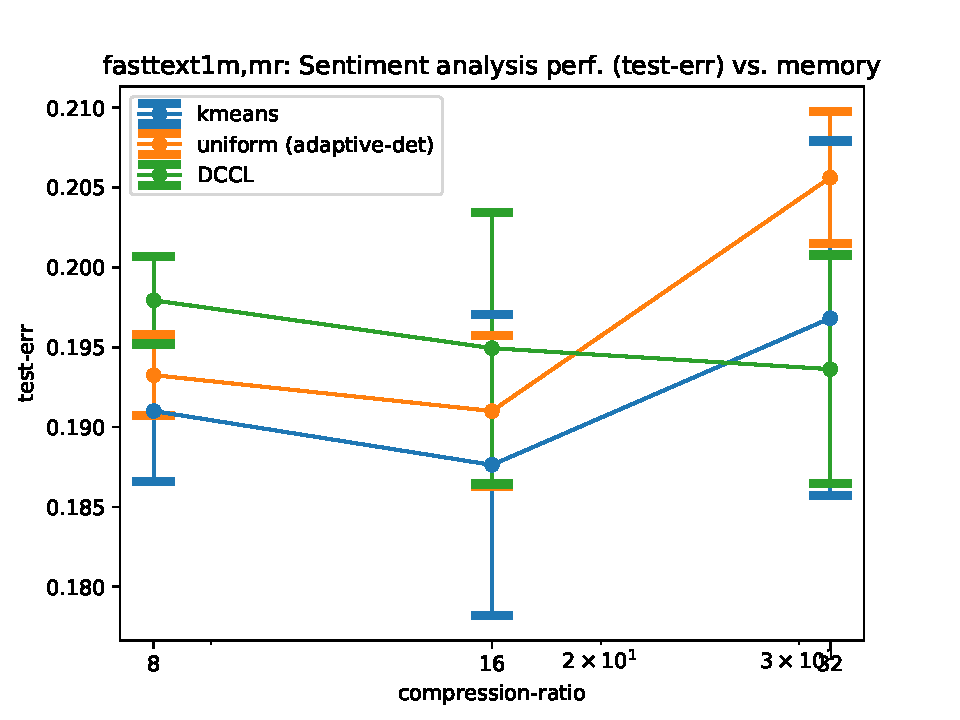
\includegraphics[width=0.28\linewidth]{figures/fasttext1m_mr_test-err_vs_compression.pdf} &
%	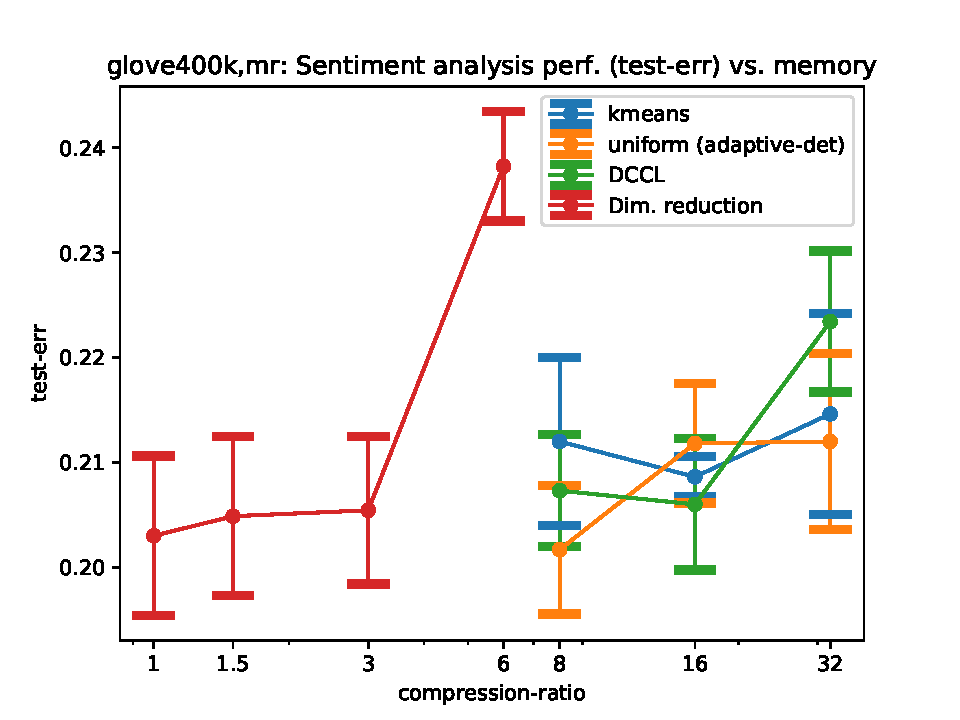
\includegraphics[width=0.28\linewidth]{figures/glove400k_mr_test-err_vs_compression.pdf} &
%	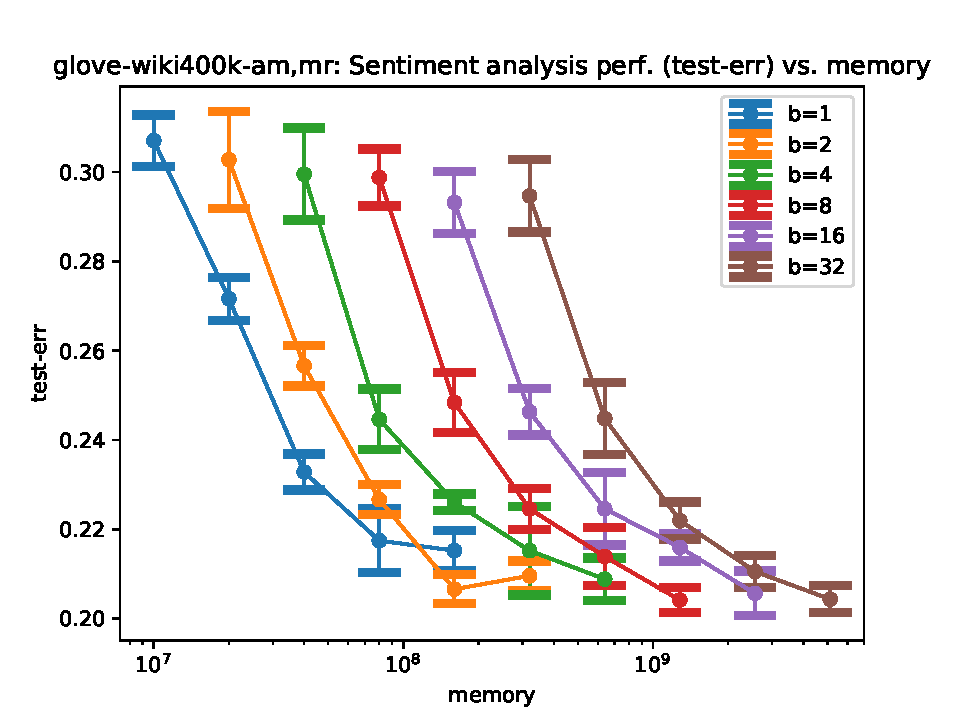
\includegraphics[width=0.28\linewidth]{figures/glove-wiki400k-am_mr_test-err_vs_compression.pdf} \\[-0.5em]
%	\end{tabular}
%	\caption{
%		Sentiment analysis results for different embeddings methods (pre-trained fastText and GloVe embeddings, and GloVe embeddings trained from scratch), on different sentiment analysis datasets (MPQA, TREC, SST, CR, SUBJ, MR).
%	}
%	\label{fig:all_sentiment}
%\end{figure}
%
%\begin{figure*}
%	\centering
%	%	\begin{tabular}{c c c c}
%	\begin{tabular}{@{\hskip -0.0in}c@{\hskip -0.0in}c@{\hskip -0.0in}c@{\hskip -0.0in}c@{\hskip -0.0in}}
%		EIG-OVERLAP & . & . & . \\
%		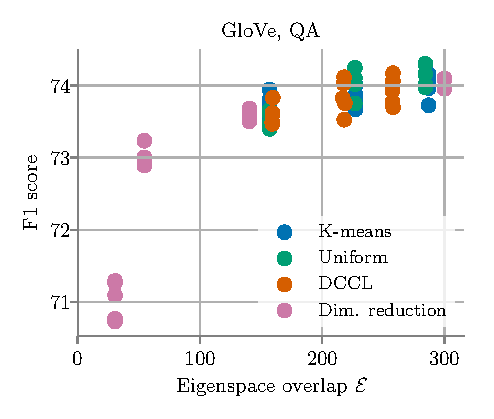
\includegraphics[width=.245\linewidth]{figures/glove400k_qa_best-f1_vs_subspace-eig-overlap_linx.pdf} &
%		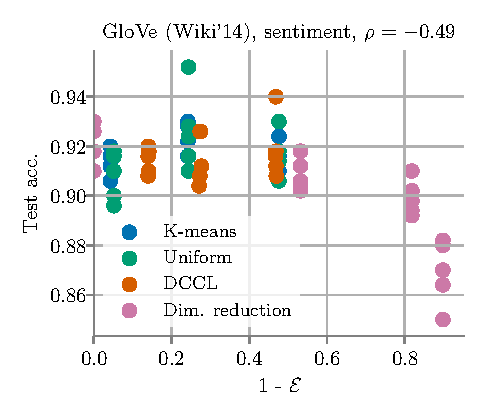
\includegraphics[width=.245\linewidth]{figures/glove400k_sentiment_trec_test-acc_vs_subspace-eig-overlap_linx.pdf} &
%		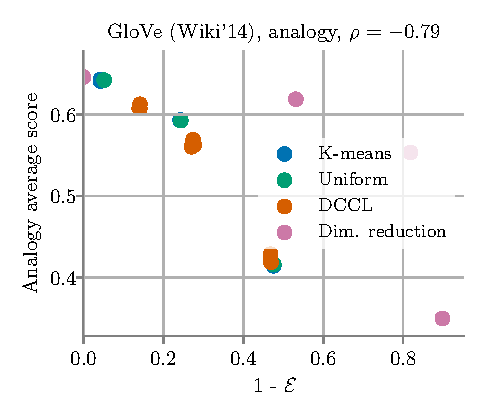
\includegraphics[width=.245\linewidth]{figures/glove400k_intrinsics_analogy-avg-score_vs_subspace-eig-overlap_linx.pdf} &
%		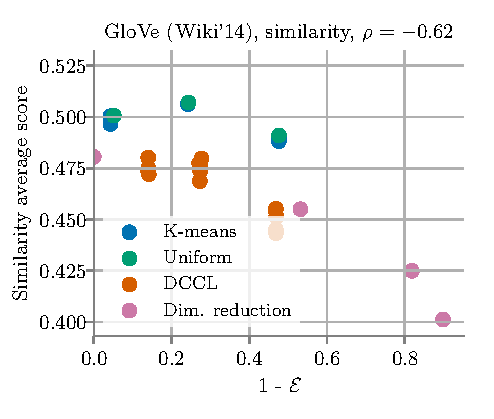
\includegraphics[width=.245\linewidth]{figures/glove400k_intrinsics_similarity-avg-score_vs_subspace-eig-overlap_linx.pdf} \\
%		
%		EIG-DISTANCE & . & . & . \\
%		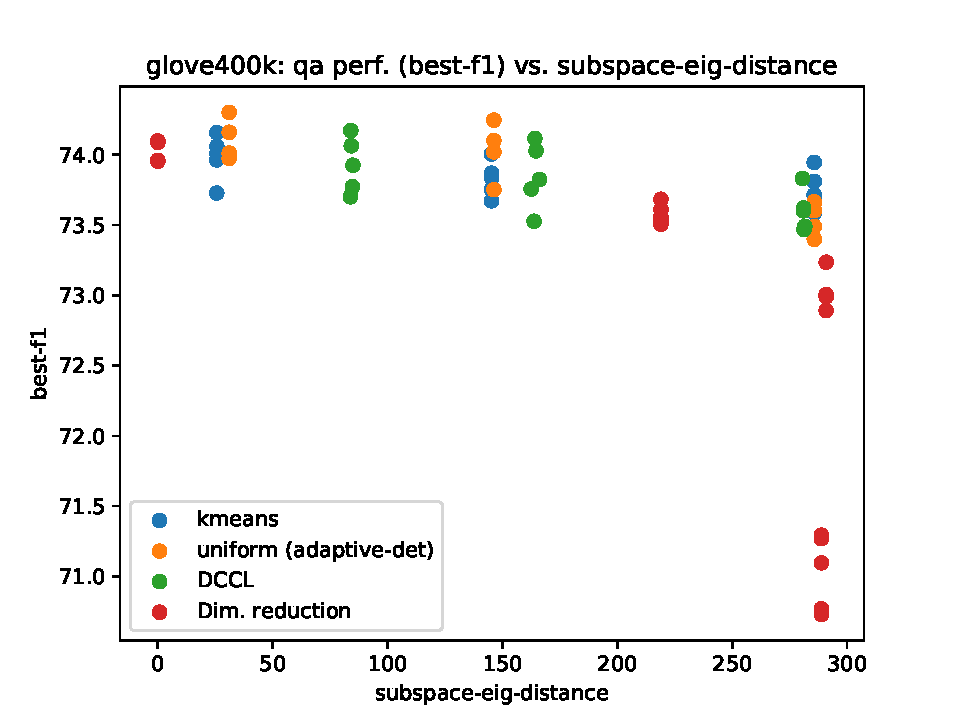
\includegraphics[width=.245\linewidth]{figures/glove400k_qa_best-f1_vs_subspace-eig-distance_linx.pdf} &
%		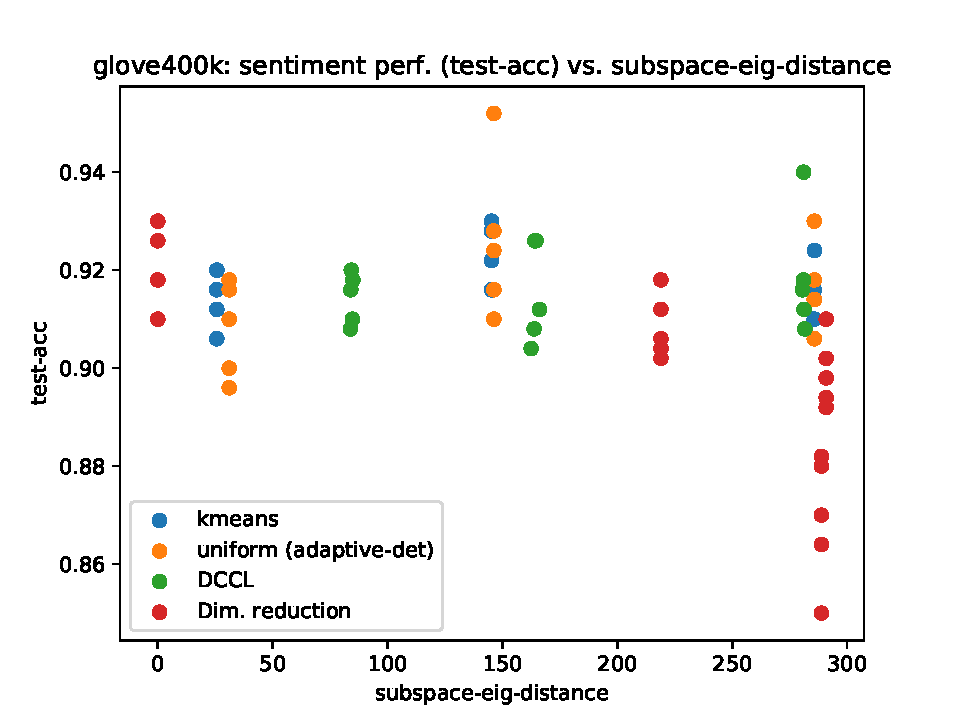
\includegraphics[width=.245\linewidth]{figures/glove400k_sentiment_trec_test-acc_vs_subspace-eig-distance_linx.pdf} &
%		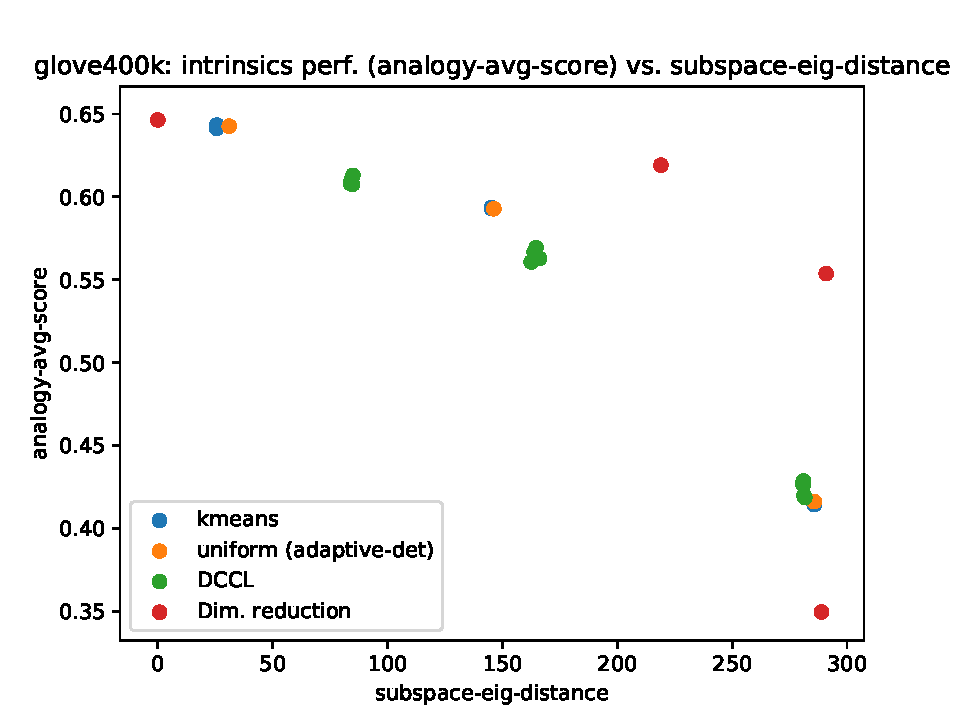
\includegraphics[width=.245\linewidth]{figures/glove400k_intrinsics_analogy-avg-score_vs_subspace-eig-distance_linx.pdf} &
%		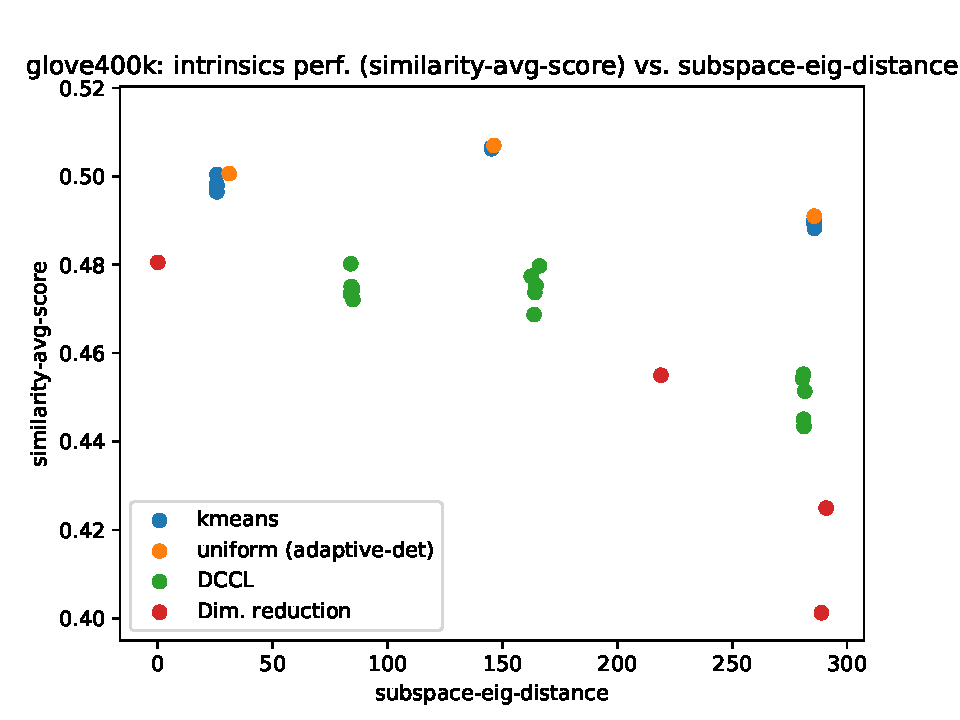
\includegraphics[width=.245\linewidth]{figures/glove400k_intrinsics_similarity-avg-score_vs_subspace-eig-distance_linx.pdf} \\
%		
%		FROBENIUS ERROR & . & . & . \\		
%		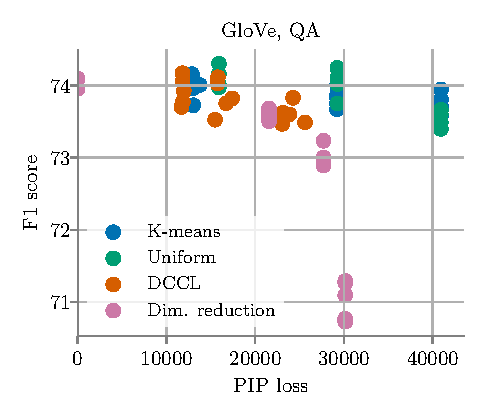
\includegraphics[width=.245\linewidth]{figures/glove400k_qa_best-f1_vs_gram-large-dim-frob-error_linx.pdf} &
%		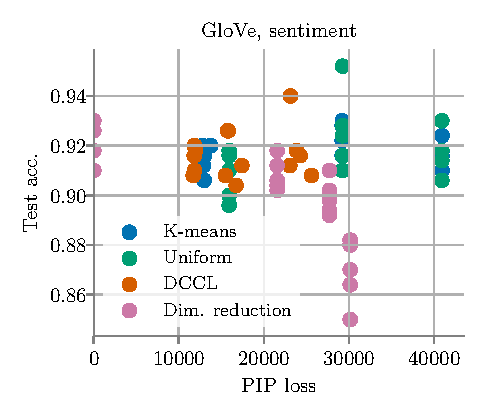
\includegraphics[width=.245\linewidth]{figures/glove400k_sentiment_trec_test-acc_vs_gram-large-dim-frob-error_linx.pdf} &
%		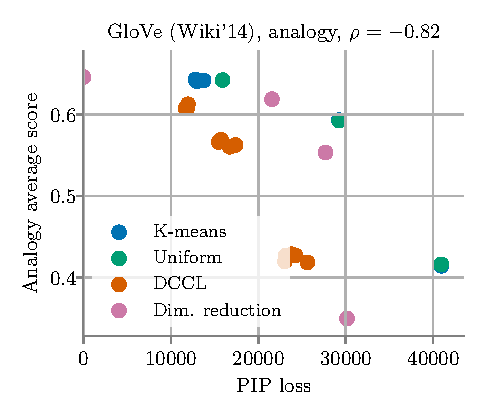
\includegraphics[width=.245\linewidth]{figures/glove400k_intrinsics_analogy-avg-score_vs_gram-large-dim-frob-error_linx.pdf} &
%		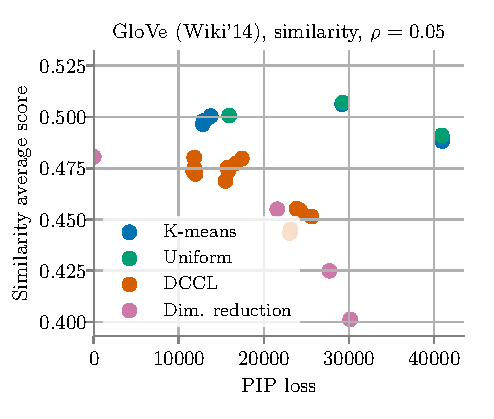
\includegraphics[width=.245\linewidth]{figures/glove400k_intrinsics_similarity-avg-score_vs_gram-large-dim-frob-error_linx.pdf} \\
%		
%		RECONSTRUCTION ERROR (FROB) & . & . & . \\		
%		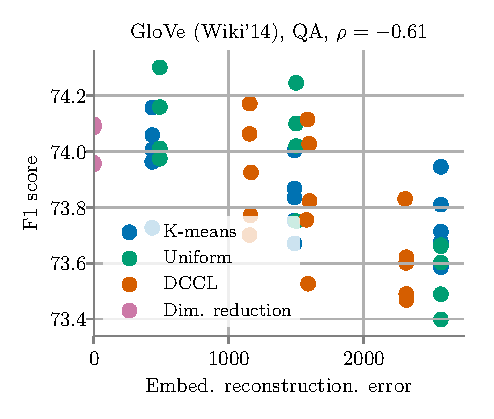
\includegraphics[width=.245\linewidth]{figures/glove400k_qa_best-f1_vs_embed-frob-error_linx.pdf} &
%		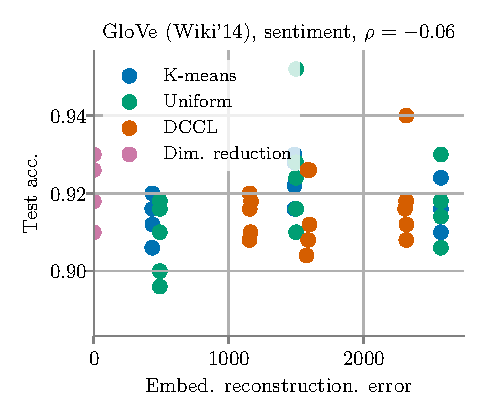
\includegraphics[width=.245\linewidth]{figures/glove400k_sentiment_trec_test-acc_vs_embed-frob-error_linx.pdf} &
%		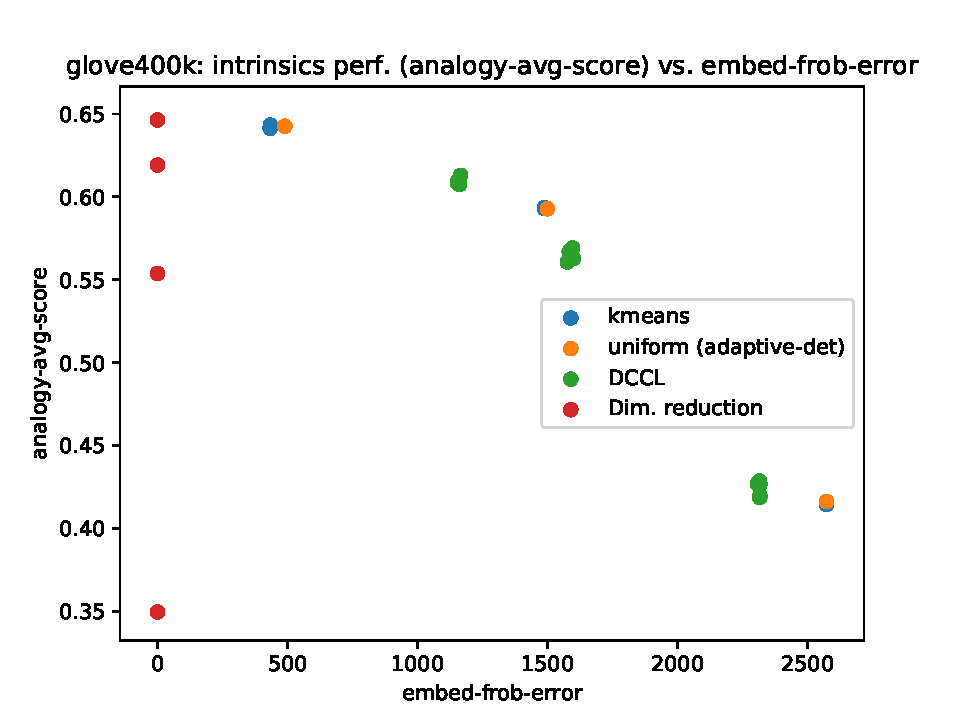
\includegraphics[width=.245\linewidth]{figures/glove400k_intrinsics_analogy-avg-score_vs_embed-frob-error_linx.pdf} &
%		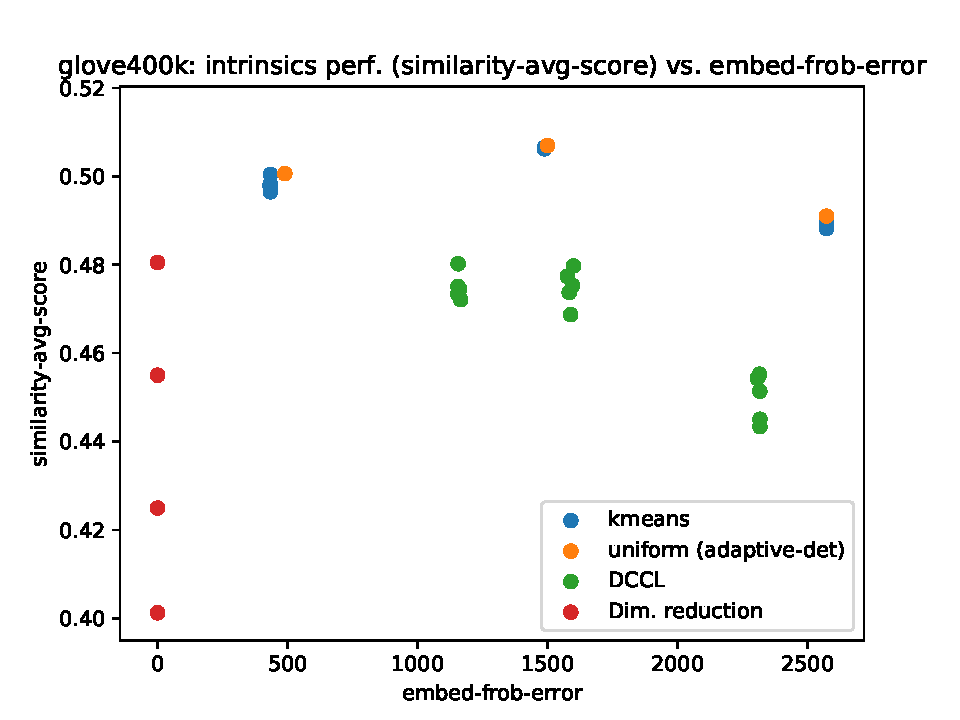
\includegraphics[width=.245\linewidth]{figures/glove400k_intrinsics_similarity-avg-score_vs_embed-frob-error_linx.pdf} \\
%		
%		
%		%DELTA1 (Lambda = sigma min/100) & . & . & . \\
%		%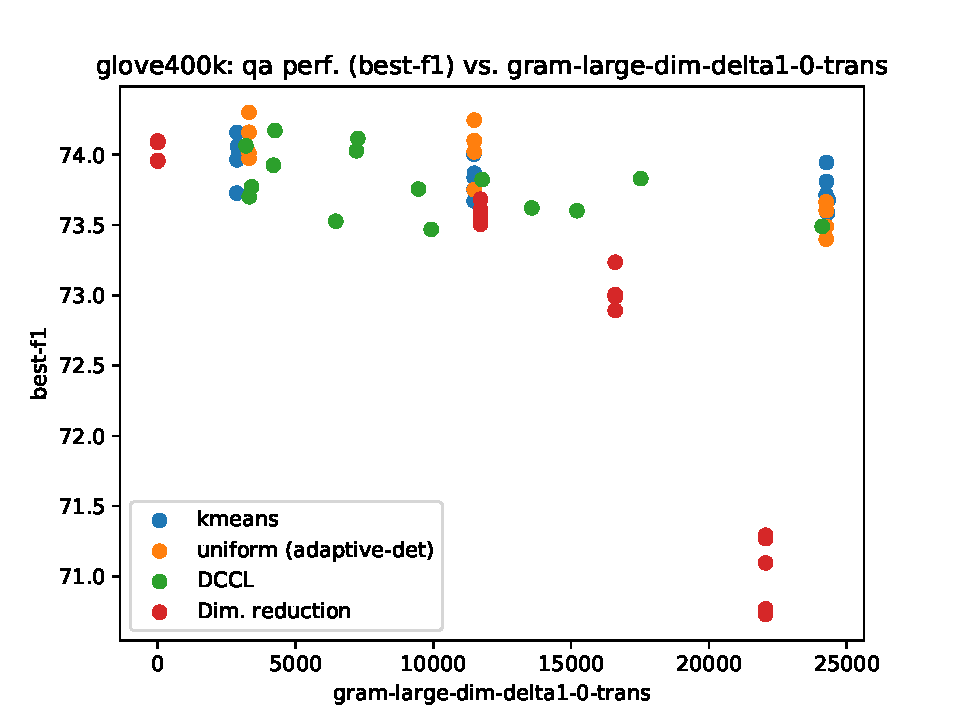
\includegraphics[width=.245\linewidth]{figures/glove400k_qa_best-f1_vs_gram-large-dim-delta1-0-trans_linx.pdf} &
%		%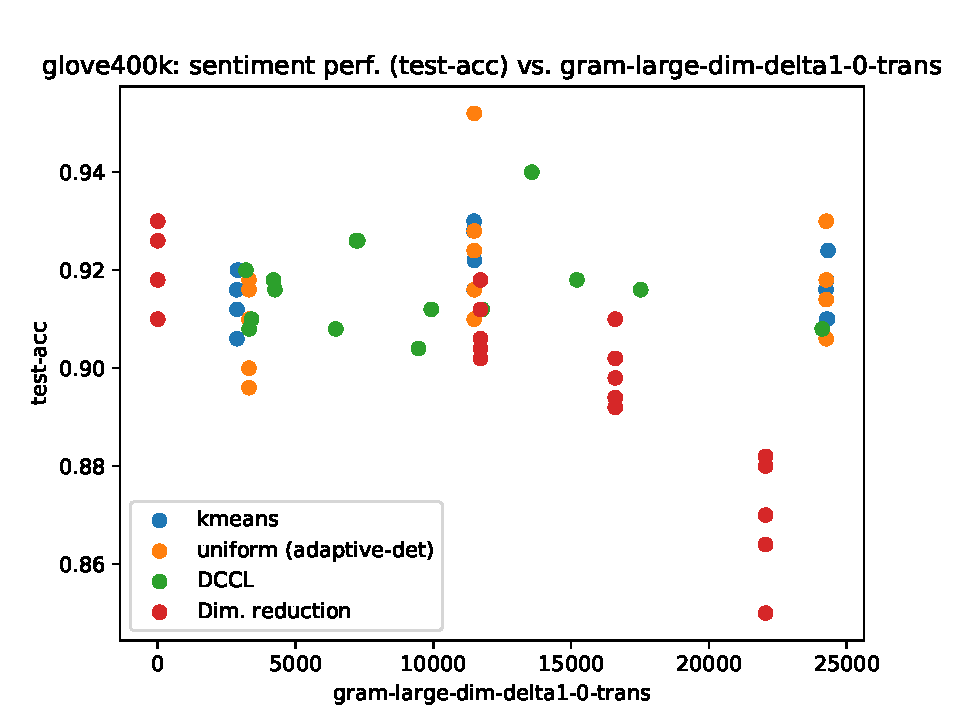
\includegraphics[width=.245\linewidth]{figures/glove400k_sentiment_trec_test-acc_vs_gram-large-dim-delta1-0-trans_linx.pdf} &
%		%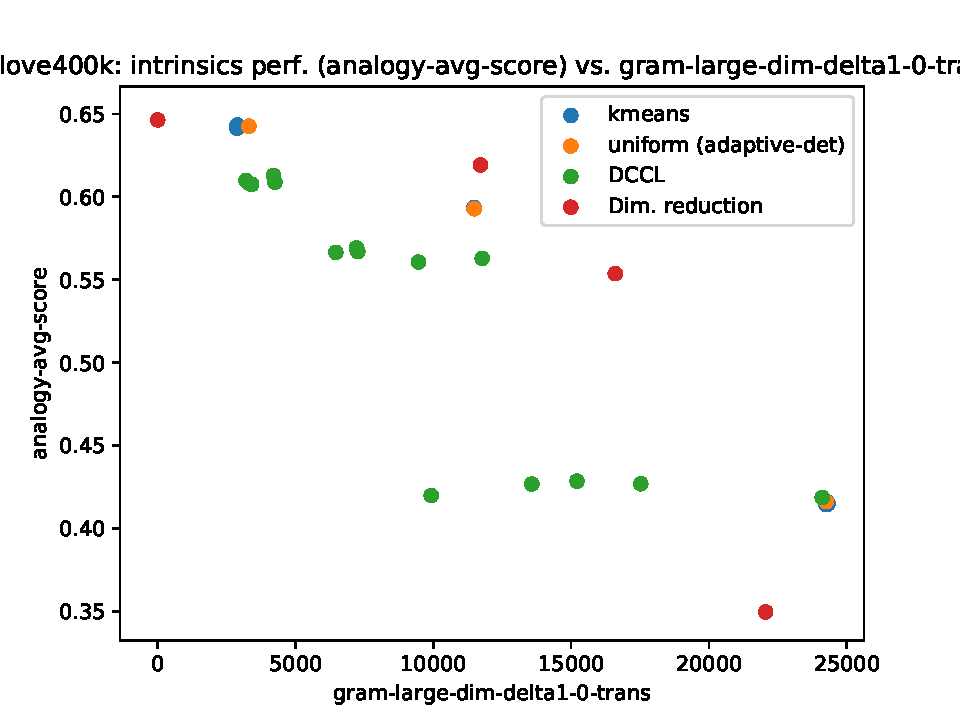
\includegraphics[width=.245\linewidth]{figures/glove400k_intrinsics_analogy-avg-score_vs_gram-large-dim-delta1-0-trans_linx.pdf} &
%		%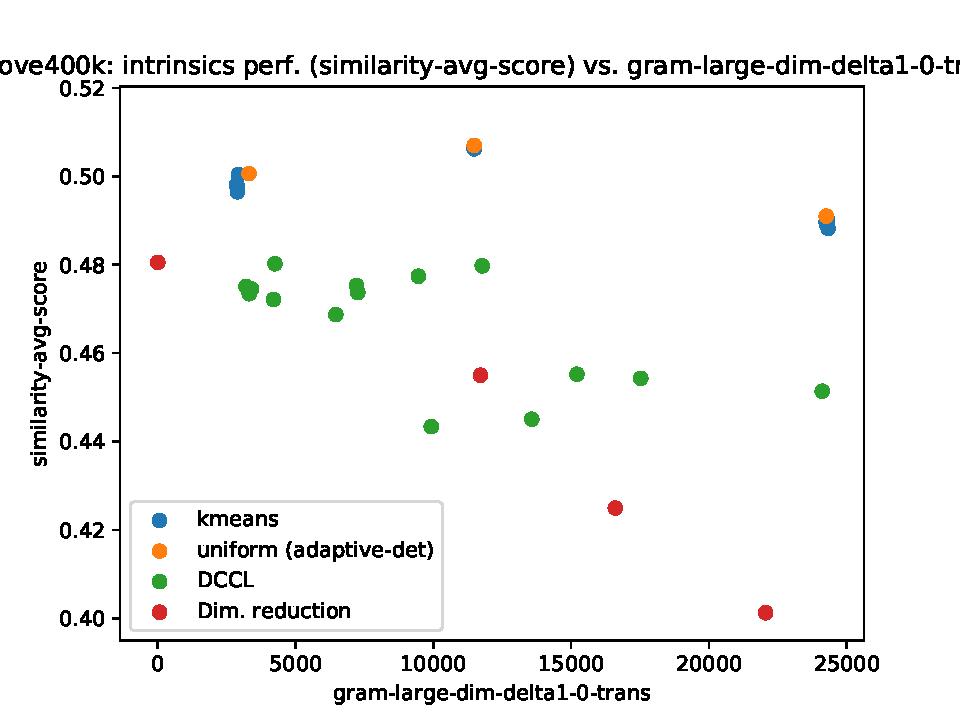
\includegraphics[width=.245\linewidth]{figures/glove400k_intrinsics_similarity-avg-score_vs_gram-large-dim-delta1-0-trans_linx.pdf} \\
%		
%		DELTA1 (Lambda = sigma min) & . & . & . \\
%		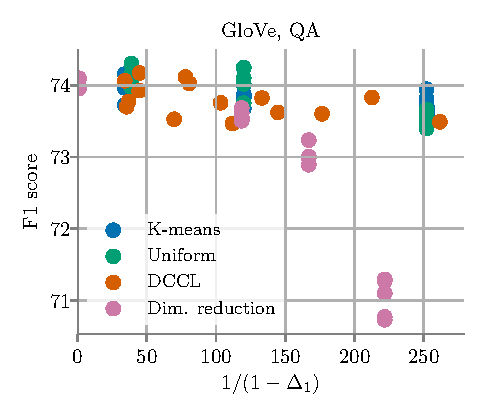
\includegraphics[width=.245\linewidth]{figures/glove400k_qa_best-f1_vs_gram-large-dim-delta1-2-trans_linx.pdf} &
%		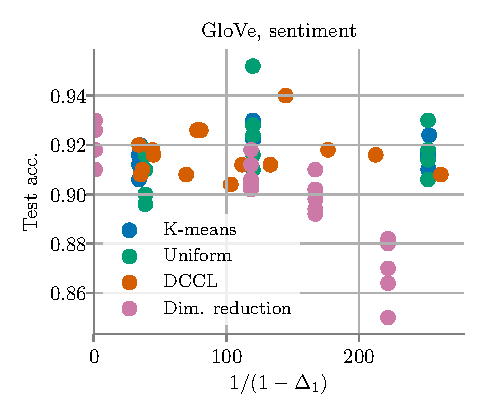
\includegraphics[width=.245\linewidth]{figures/glove400k_sentiment_trec_test-acc_vs_gram-large-dim-delta1-2-trans_linx.pdf} &
%		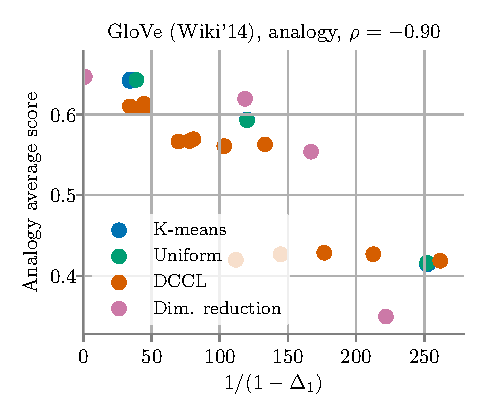
\includegraphics[width=.245\linewidth]{figures/glove400k_intrinsics_analogy-avg-score_vs_gram-large-dim-delta1-2-trans_linx.pdf} &
%		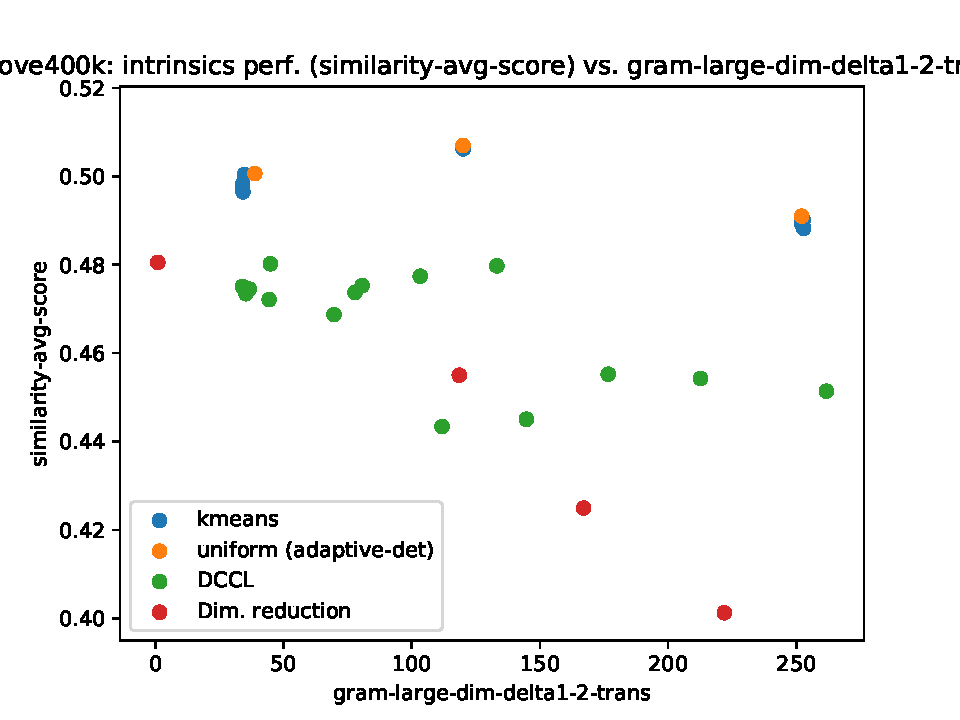
\includegraphics[width=.245\linewidth]{figures/glove400k_intrinsics_similarity-avg-score_vs_gram-large-dim-delta1-2-trans_linx.pdf} \\		
%		
%		DELTA1 (lambda = sigma max) & . & . & . \\
%		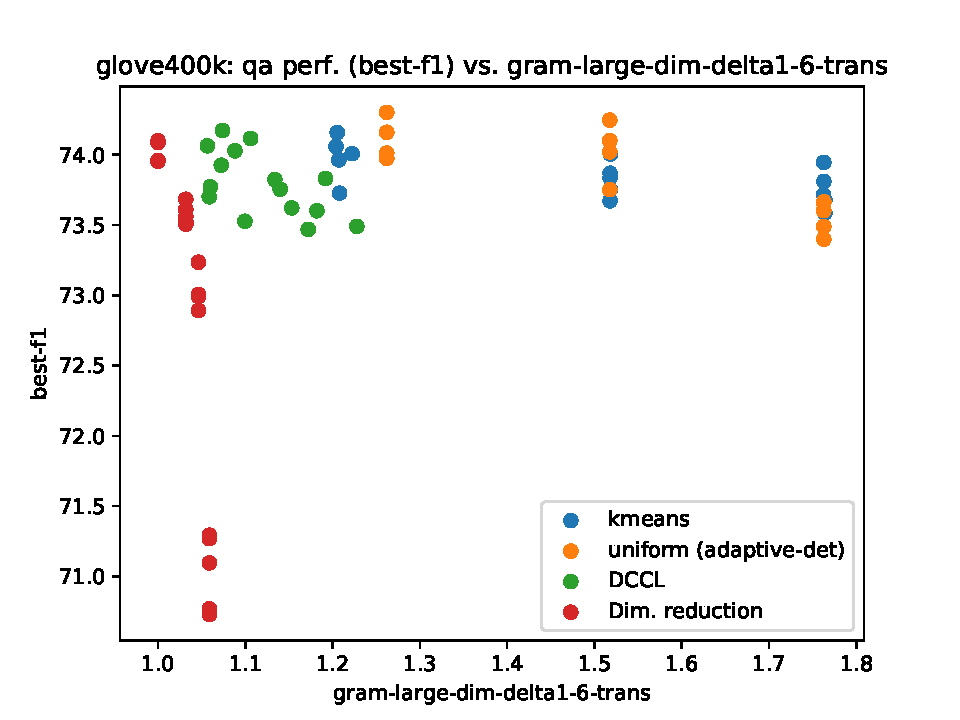
\includegraphics[width=.245\linewidth]{figures/glove400k_qa_best-f1_vs_gram-large-dim-delta1-6-trans_linx.pdf} &
%		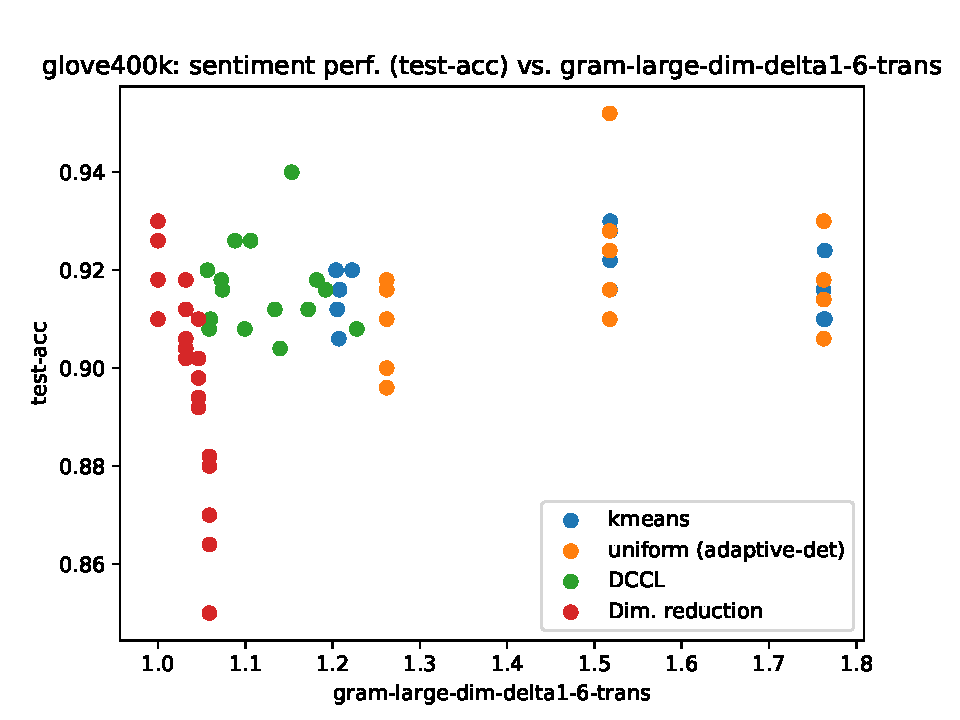
\includegraphics[width=.245\linewidth]{figures/glove400k_sentiment_trec_test-acc_vs_gram-large-dim-delta1-6-trans_linx.pdf} &
%		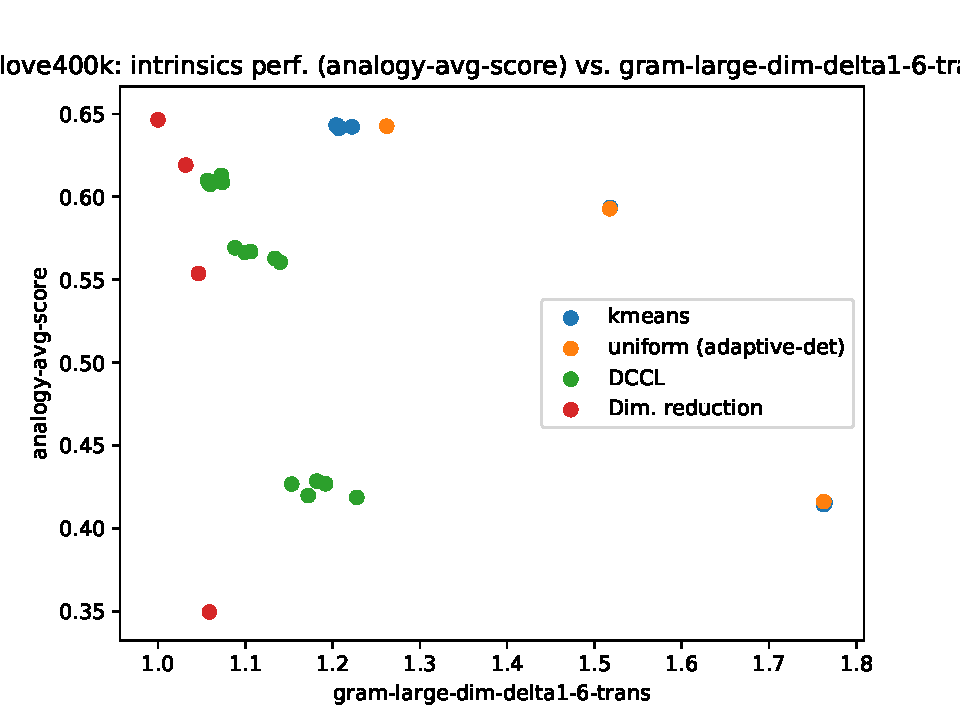
\includegraphics[width=.245\linewidth]{figures/glove400k_intrinsics_analogy-avg-score_vs_gram-large-dim-delta1-6-trans_linx.pdf} &
%		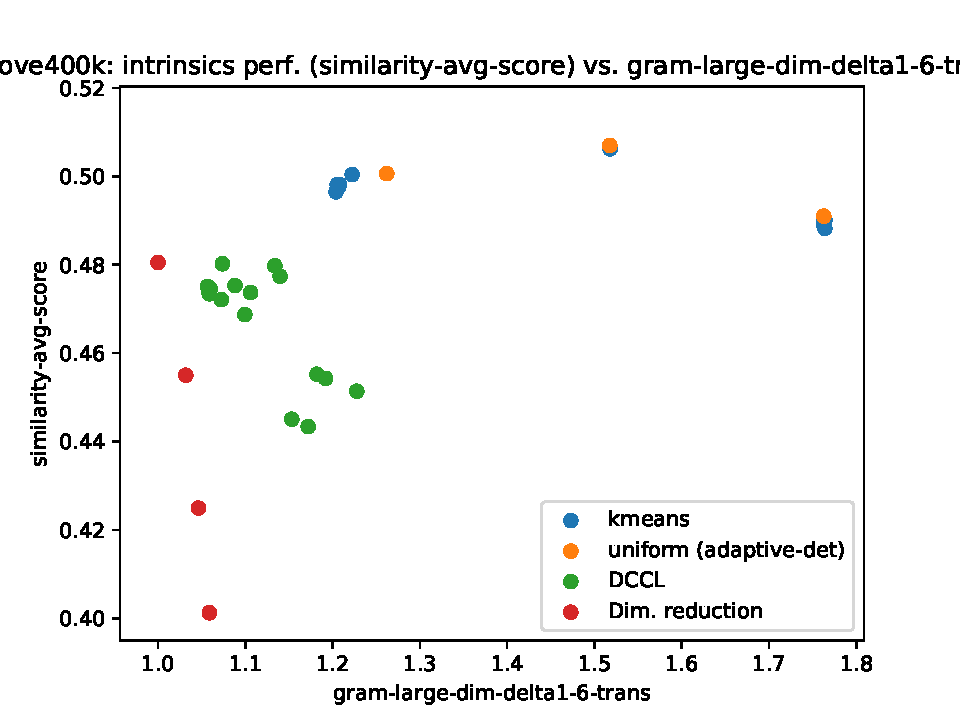
\includegraphics[width=.245\linewidth]{figures/glove400k_intrinsics_similarity-avg-score_vs_gram-large-dim-delta1-6-trans_linx.pdf} \\		
%		
%		\;\;\;\;\;(a) & \;\;\;\;\;\;(b) & \;\;\;\;\;\;(c) & \;\;\;\;\;\;(d)
%	\end{tabular}
%	\caption{GLOVE400k: Performance vs. metrics. (a) QA, (b) Sentiment (TREC), (c) Analogy average, (d) Similarity average.
%	}
%	\label{fig:glove400k_comparison_results}
%\end{figure*}
%
%
%\begin{figure*}
%	\centering
%	%	\begin{tabular}{c c c c}
%	\begin{tabular}{@{\hskip -0.0in}c@{\hskip -0.0in}c@{\hskip -0.0in}c@{\hskip -0.0in}c@{\hskip -0.0in}}
%		EIG-OVERLAP & . & . & . \\
%		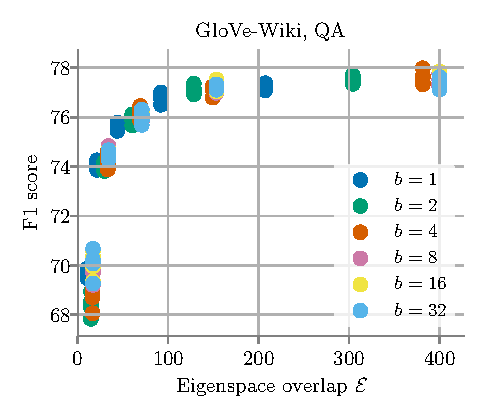
\includegraphics[width=.245\linewidth]{figures/glove-wiki400k-am_qa_best-f1_vs_subspace-eig-overlap_linx.pdf} &
%		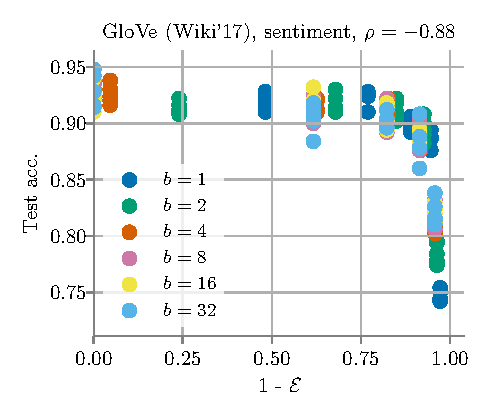
\includegraphics[width=.245\linewidth]{figures/glove-wiki400k-am_sentiment_trec_test-acc_vs_subspace-eig-overlap_linx.pdf} &
%		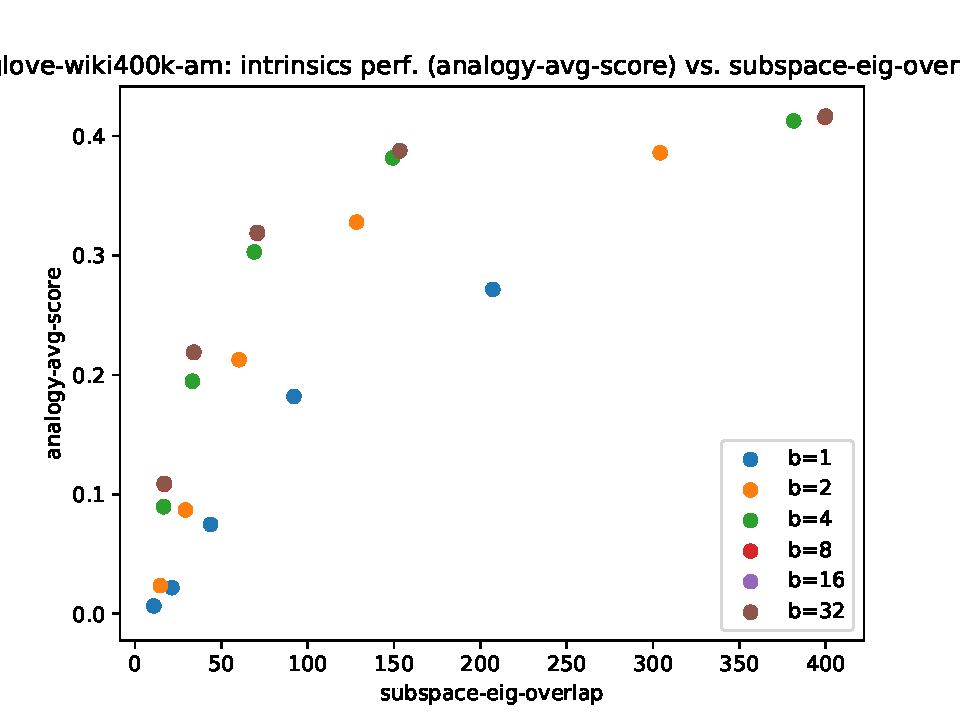
\includegraphics[width=.245\linewidth]{figures/glove-wiki400k-am_intrinsics_analogy-avg-score_vs_subspace-eig-overlap_linx.pdf} &
%		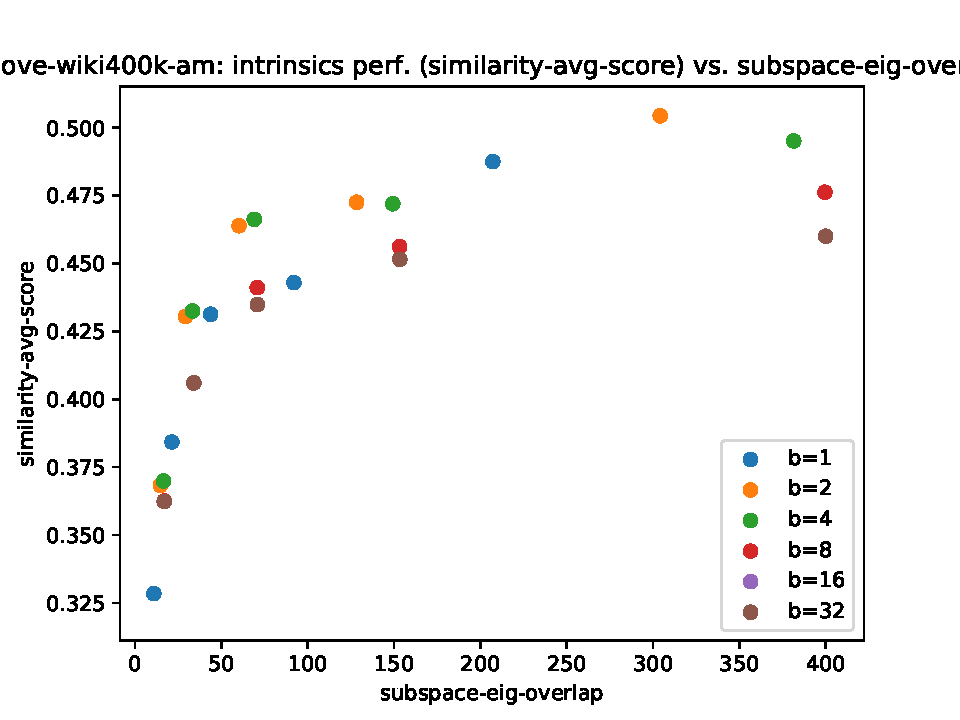
\includegraphics[width=.245\linewidth]{figures/glove-wiki400k-am_intrinsics_similarity-avg-score_vs_subspace-eig-overlap_linx.pdf} \\
%		
%		EIG-DISTANCE & . & . & . \\
%		\includegraphics[width=.245\linewidth]{figures/glove-wiki400k-am_qa_best-f1_vs_subspace-eig-distance_linx.pdf} &
%		\includegraphics[width=.245\linewidth]{figures/glove-wiki400k-am_sentiment_trec_test-acc_vs_subspace-eig-distance_linx.pdf} &
%		\includegraphics[width=.245\linewidth]{figures/glove-wiki400k-am_intrinsics_analogy-avg-score_vs_subspace-eig-distance_linx.pdf} &
%		\includegraphics[width=.245\linewidth]{figures/glove-wiki400k-am_intrinsics_similarity-avg-score_vs_subspace-eig-distance_linx.pdf} \\
%		
%		FROBENIUS ERROR & . & . & . \\		
%		\includegraphics[width=.245\linewidth]{figures/glove-wiki400k-am_qa_best-f1_vs_gram-large-dim-frob-error_linx.pdf} &
%		\includegraphics[width=.245\linewidth]{figures/glove-wiki400k-am_sentiment_trec_test-acc_vs_gram-large-dim-frob-error_linx.pdf} &
%		\includegraphics[width=.245\linewidth]{figures/glove-wiki400k-am_intrinsics_analogy-avg-score_vs_gram-large-dim-frob-error_linx.pdf} &
%		\includegraphics[width=.245\linewidth]{figures/glove-wiki400k-am_intrinsics_similarity-avg-score_vs_gram-large-dim-frob-error_linx.pdf} \\
%		
%		
%		RECONSTRUCTION ERROR (FROB) & . & . & . \\		
%		\includegraphics[width=.245\linewidth]{figures/glove-wiki400k-am_qa_best-f1_vs_embed-frob-error_linx.pdf} &
%		\includegraphics[width=.245\linewidth]{figures/glove-wiki400k-am_sentiment_trec_test-acc_vs_embed-frob-error_linx.pdf} &
%		\includegraphics[width=.245\linewidth]{figures/glove-wiki400k-am_intrinsics_analogy-avg-score_vs_embed-frob-error_linx.pdf} &
%		\includegraphics[width=.245\linewidth]{figures/glove-wiki400k-am_intrinsics_similarity-avg-score_vs_embed-frob-error_linx.pdf} \\
%		%		DELTA1 (Lambda = sigma min/100) & . & . & . \\
%		%		\includegraphics[width=.245\linewidth]{figures/glove-wiki400k-am_qa_best-f1_vs_gram-large-dim-delta1-0-trans_linx.pdf} &
%		%		\includegraphics[width=.245\linewidth]{figures/glove-wiki400k-am_sentiment_trec_test-acc_vs_gram-large-dim-delta1-0-trans_linx.pdf} &
%		%		\includegraphics[width=.245\linewidth]{figures/glove-wiki400k-am_intrinsics_analogy-avg-score_vs_gram-large-dim-delta1-0-trans_linx.pdf} &
%		%		\includegraphics[width=.245\linewidth]{figures/glove-wiki400k-am_intrinsics_similarity-avg-score_vs_gram-large-dim-delta1-0-trans_linx.pdf} \\		
%		
%		DELTA1 (Lambda = sigma min) & . & . & . \\
%		\includegraphics[width=.245\linewidth]{figures/glove-wiki400k-am_qa_best-f1_vs_gram-large-dim-delta1-2-trans_linx.pdf} &
%		\includegraphics[width=.245\linewidth]{figures/glove-wiki400k-am_sentiment_trec_test-acc_vs_gram-large-dim-delta1-2-trans_linx.pdf} &
%		\includegraphics[width=.245\linewidth]{figures/glove-wiki400k-am_intrinsics_analogy-avg-score_vs_gram-large-dim-delta1-2-trans_linx.pdf} &
%		\includegraphics[width=.245\linewidth]{figures/glove-wiki400k-am_intrinsics_similarity-avg-score_vs_gram-large-dim-delta1-2-trans_linx.pdf} \\		
%		
%		DELTA1 (lambda = sigma max) & . & . & . \\
%		\includegraphics[width=.245\linewidth]{figures/glove-wiki400k-am_qa_best-f1_vs_gram-large-dim-delta1-6-trans_linx.pdf} &
%		\includegraphics[width=.245\linewidth]{figures/glove-wiki400k-am_sentiment_trec_test-acc_vs_gram-large-dim-delta1-6-trans_linx.pdf} &
%		\includegraphics[width=.245\linewidth]{figures/glove-wiki400k-am_intrinsics_analogy-avg-score_vs_gram-large-dim-delta1-6-trans_linx.pdf} &
%		\includegraphics[width=.245\linewidth]{figures/glove-wiki400k-am_intrinsics_similarity-avg-score_vs_gram-large-dim-delta1-6-trans_linx.pdf} \\		
%		
%		\;\;\;\;\;(a) & \;\;\;\;\;\;(b) & \;\;\;\;\;\;(c) & \;\;\;\;\;\;(d)
%	\end{tabular}
%	\caption{glove-wiki400k-am: Performance vs. metrics. (a) QA, (b) Sentiment (TREC), (c) Analogy average, (d) Similarity average.
%	}
%	\label{fig:glove_wiki400k_am_comparison_results}
%\end{figure*}
%
%
%\begin{figure*}
%	\centering
%	%	\begin{tabular}{c c c c}
%	\begin{tabular}{@{\hskip -0.0in}c@{\hskip -0.0in}c@{\hskip -0.0in}c@{\hskip -0.0in}c@{\hskip -0.0in}}
%		EIG-OVERLAP & . & . & . \\
%		\includegraphics[width=.245\linewidth]{figures/fasttext1m_qa_best-f1_vs_subspace-eig-overlap_linx.pdf} &
%		\includegraphics[width=.245\linewidth]{figures/fasttext1m_sentiment_trec_test-acc_vs_subspace-eig-overlap_linx.pdf} &
%		\includegraphics[width=.245\linewidth]{figures/fasttext1m_intrinsics_analogy-avg-score_vs_subspace-eig-overlap_linx.pdf} &
%		\includegraphics[width=.245\linewidth]{figures/fasttext1m_intrinsics_similarity-avg-score_vs_subspace-eig-overlap_linx.pdf} \\
%		
%		EIG-DISTANCE & . & . & . \\
%		\includegraphics[width=.245\linewidth]{figures/fasttext1m_qa_best-f1_vs_subspace-eig-distance_linx.pdf} &
%		\includegraphics[width=.245\linewidth]{figures/fasttext1m_sentiment_trec_test-acc_vs_subspace-eig-distance_linx.pdf} &
%		\includegraphics[width=.245\linewidth]{figures/fasttext1m_intrinsics_analogy-avg-score_vs_subspace-eig-distance_linx.pdf} &
%		\includegraphics[width=.245\linewidth]{figures/fasttext1m_intrinsics_similarity-avg-score_vs_subspace-eig-distance_linx.pdf} \\
%		
%		FROBENIUS ERROR & . & . & . \\		
%		\includegraphics[width=.245\linewidth]{figures/fasttext1m_qa_best-f1_vs_gram-large-dim-frob-error_linx.pdf} &
%		\includegraphics[width=.245\linewidth]{figures/fasttext1m_sentiment_trec_test-acc_vs_gram-large-dim-frob-error_linx.pdf} &
%		\includegraphics[width=.245\linewidth]{figures/fasttext1m_intrinsics_analogy-avg-score_vs_gram-large-dim-frob-error_linx.pdf} &
%		\includegraphics[width=.245\linewidth]{figures/fasttext1m_intrinsics_similarity-avg-score_vs_gram-large-dim-frob-error_linx.pdf} \\
%		
%		
%		RECONSTRUCTION ERROR (FROB) & . & . & . \\		
%		\includegraphics[width=.245\linewidth]{figures/fasttext1m_qa_best-f1_vs_embed-frob-error_linx.pdf} &
%		\includegraphics[width=.245\linewidth]{figures/fasttext1m_sentiment_trec_test-acc_vs_embed-frob-error_linx.pdf} &
%		\includegraphics[width=.245\linewidth]{figures/fasttext1m_intrinsics_analogy-avg-score_vs_embed-frob-error_linx.pdf} &
%		\includegraphics[width=.245\linewidth]{figures/fasttext1m_intrinsics_similarity-avg-score_vs_embed-frob-error_linx.pdf} \\
%		%		DELTA1 (Tiny lambda) & . & . & . \\
%		%		\includegraphics[width=.245\linewidth]{figures/fasttext1m_qa_best-f1_vs_gram-large-dim-delta1-0-trans_linx.pdf} &
%		%		\includegraphics[width=.245\linewidth]{figures/fasttext1m_sentiment_trec_test-acc_vs_gram-large-dim-delta1-0-trans_linx.pdf} &
%		%		\includegraphics[width=.245\linewidth]{figures/fasttext1m_intrinsics_analogy-avg-score_vs_gram-large-dim-delta1-0-trans_linx.pdf} &
%		%		\includegraphics[width=.245\linewidth]{figures/fasttext1m_intrinsics_similarity-avg-score_vs_gram-large-dim-delta1-0-trans_linx.pdf} \\		
%		
%		DELTA1 (Tiny lambda) & . & . & . \\
%		\includegraphics[width=.245\linewidth]{figures/fasttext1m_qa_best-f1_vs_gram-large-dim-delta1-2-trans_linx.pdf} &
%		\includegraphics[width=.245\linewidth]{figures/fasttext1m_sentiment_trec_test-acc_vs_gram-large-dim-delta1-2-trans_linx.pdf} &
%		\includegraphics[width=.245\linewidth]{figures/fasttext1m_intrinsics_analogy-avg-score_vs_gram-large-dim-delta1-2-trans_linx.pdf} &
%		\includegraphics[width=.245\linewidth]{figures/fasttext1m_intrinsics_similarity-avg-score_vs_gram-large-dim-delta1-2-trans_linx.pdf} \\		
%		
%		DELTA1 (lambda = sigma max) & . & . & . \\
%		\includegraphics[width=.245\linewidth]{figures/fasttext1m_qa_best-f1_vs_gram-large-dim-delta1-6-trans_linx.pdf} &
%		\includegraphics[width=.245\linewidth]{figures/fasttext1m_sentiment_trec_test-acc_vs_gram-large-dim-delta1-6-trans_linx.pdf} &
%		\includegraphics[width=.245\linewidth]{figures/fasttext1m_intrinsics_analogy-avg-score_vs_gram-large-dim-delta1-6-trans_linx.pdf} &
%		\includegraphics[width=.245\linewidth]{figures/fasttext1m_intrinsics_similarity-avg-score_vs_gram-large-dim-delta1-6-trans_linx.pdf} \\		
%		
%		\;\;\;\;\;(a) & \;\;\;\;\;\;(b) & \;\;\;\;\;\;(c) & \;\;\;\;\;\;(d)
%	\end{tabular}
%	\caption{fasttext1m: Performance vs. metrics. (a) QA, (b) Sentiment (TREC), (c) Analogy average, (d) Similarity average.
%	}
%	\label{fig:fasttext1m_comparison_results}
%\end{figure*}
%
%
%
%% SENTIMENT ANALYSIS
%
%\begin{figure*}
%	\centering
%	%	\begin{tabular}{c c c c}
%	\begin{tabular}{@{\hskip -0.0in}c@{\hskip -0.0in}c@{\hskip -0.0in}c@{\hskip -0.0in}c@{\hskip -0.0in}c@{\hskip -0.0in}}
%		EIG-OVERLAP & . & . & . & .\\
%		\includegraphics[width=.2\linewidth]{figures/glove400k_sentiment_mr_test-acc_vs_subspace-eig-overlap_linx.pdf} &
%		\includegraphics[width=.2\linewidth]{figures/glove400k_sentiment_subj_test-acc_vs_subspace-eig-overlap_linx.pdf} &
%		\includegraphics[width=.2\linewidth]{figures/glove400k_sentiment_cr_test-acc_vs_subspace-eig-overlap_linx.pdf} &
%		\includegraphics[width=.2\linewidth]{figures/glove400k_sentiment_sst_test-acc_vs_subspace-eig-overlap_linx.pdf} &
%		\includegraphics[width=.2\linewidth]{figures/glove400k_sentiment_mpqa_test-acc_vs_subspace-eig-overlap_linx.pdf} \\
%		
%		EIG-DISTANCE & . & . & . & .\\
%		\includegraphics[width=.2\linewidth]{figures/glove400k_sentiment_mr_test-acc_vs_subspace-eig-distance_linx.pdf} &
%		\includegraphics[width=.2\linewidth]{figures/glove400k_sentiment_subj_test-acc_vs_subspace-eig-distance_linx.pdf} &
%		\includegraphics[width=.2\linewidth]{figures/glove400k_sentiment_cr_test-acc_vs_subspace-eig-distance_linx.pdf} &
%		\includegraphics[width=.2\linewidth]{figures/glove400k_sentiment_sst_test-acc_vs_subspace-eig-distance_linx.pdf} &
%		\includegraphics[width=.2\linewidth]{figures/glove400k_sentiment_mpqa_test-acc_vs_subspace-eig-distance_linx.pdf} \\
%		
%		
%		FROBENIUS ERROR & . & . & . & .\\
%		\includegraphics[width=.2\linewidth]{figures/glove400k_sentiment_mr_test-acc_vs_gram-large-dim-frob-error_linx.pdf} &
%		\includegraphics[width=.2\linewidth]{figures/glove400k_sentiment_subj_test-acc_vs_gram-large-dim-frob-error_linx.pdf} &
%		\includegraphics[width=.2\linewidth]{figures/glove400k_sentiment_cr_test-acc_vs_gram-large-dim-frob-error_linx.pdf} &
%		\includegraphics[width=.2\linewidth]{figures/glove400k_sentiment_sst_test-acc_vs_gram-large-dim-frob-error_linx.pdf} &
%		\includegraphics[width=.2\linewidth]{figures/glove400k_sentiment_mpqa_test-acc_vs_gram-large-dim-frob-error_linx.pdf} \\
%		
%		RECONSTRUCTION ERROR (FROB) & . & . & . & .\\
%		\includegraphics[width=.2\linewidth]{figures/glove400k_sentiment_mr_test-acc_vs_embed-frob-error_linx.pdf} &
%		\includegraphics[width=.2\linewidth]{figures/glove400k_sentiment_subj_test-acc_vs_embed-frob-error_linx.pdf} &
%		\includegraphics[width=.2\linewidth]{figures/glove400k_sentiment_cr_test-acc_vs_embed-frob-error_linx.pdf} &
%		\includegraphics[width=.2\linewidth]{figures/glove400k_sentiment_sst_test-acc_vs_embed-frob-error_linx.pdf} &
%		\includegraphics[width=.2\linewidth]{figures/glove400k_sentiment_mpqa_test-acc_vs_embed-frob-error_linx.pdf} \\
%		
%		%		DELTA1 (Lambda = sigma min/100) & . & . & . & .\\
%		%		\includegraphics[width=.2\linewidth]{figures/glove400k_sentiment_mr_test-acc_vs_gram-large-dim-delta1-0-trans_linx.pdf} &
%		%		\includegraphics[width=.2\linewidth]{figures/glove400k_sentiment_subj_test-acc_vs_gram-large-dim-delta1-0-trans_linx.pdf} &
%		%		\includegraphics[width=.2\linewidth]{figures/glove400k_sentiment_cr_test-acc_vs_gram-large-dim-delta1-0-trans_linx.pdf} &
%		%		\includegraphics[width=.2\linewidth]{figures/glove400k_sentiment_sst_test-acc_vs_gram-large-dim-delta1-0-trans_linx.pdf} &
%		%		\includegraphics[width=.2\linewidth]{figures/glove400k_sentiment_mpqa_test-acc_vs_gram-large-dim-delta1-0-trans_linx.pdf} \\
%		
%		DELTA1 (Lambda = sigma min) & . & . & . & .\\
%		\includegraphics[width=.2\linewidth]{figures/glove400k_sentiment_mr_test-acc_vs_gram-large-dim-delta1-2-trans_linx.pdf} &
%		\includegraphics[width=.2\linewidth]{figures/glove400k_sentiment_subj_test-acc_vs_gram-large-dim-delta1-2-trans_linx.pdf} &
%		\includegraphics[width=.2\linewidth]{figures/glove400k_sentiment_cr_test-acc_vs_gram-large-dim-delta1-2-trans_linx.pdf} &
%		\includegraphics[width=.2\linewidth]{figures/glove400k_sentiment_sst_test-acc_vs_gram-large-dim-delta1-2-trans_linx.pdf} &
%		\includegraphics[width=.2\linewidth]{figures/glove400k_sentiment_mpqa_test-acc_vs_gram-large-dim-delta1-2-trans_linx.pdf} \\
%		
%		DELTA1 (Lambda = sigma max) & . & . & . & .\\
%		\includegraphics[width=.2\linewidth]{figures/glove400k_sentiment_mr_test-acc_vs_gram-large-dim-delta1-6-trans_linx.pdf} &
%		\includegraphics[width=.2\linewidth]{figures/glove400k_sentiment_subj_test-acc_vs_gram-large-dim-delta1-6-trans_linx.pdf} &
%		\includegraphics[width=.2\linewidth]{figures/glove400k_sentiment_cr_test-acc_vs_gram-large-dim-delta1-6-trans_linx.pdf} &
%		\includegraphics[width=.2\linewidth]{figures/glove400k_sentiment_sst_test-acc_vs_gram-large-dim-delta1-6-trans_linx.pdf} &
%		\includegraphics[width=.2\linewidth]{figures/glove400k_sentiment_mpqa_test-acc_vs_gram-large-dim-delta1-6-trans_linx.pdf} \\	
%		\;\;\;\;\;(a) & \;\;\;\;\;\;(b) & \;\;\;\;\;\;(c) & \;\;\;\;\;\;(d) & \;\;\;\;\;\;(e)
%	\end{tabular}
%	\caption{GLOVE400k: Performance vs. metrics, five sentiment tasks (MR, SUBJ, CR, SST, MPQA).
%	}
%	\label{fig:glove400k_sent_comparison_results}
%\end{figure*}
%
%
%
%\begin{figure*}
%	\centering
%	%	\begin{tabular}{c c c c}
%	\begin{tabular}{@{\hskip -0.0in}c@{\hskip -0.0in}c@{\hskip -0.0in}c@{\hskip -0.0in}c@{\hskip -0.0in}c@{\hskip -0.0in}}
%		EIG-OVERLAP & . & . & . & .\\
%		\includegraphics[width=.2\linewidth]{figures/glove-wiki400k-am_sentiment_mr_test-acc_vs_subspace-eig-overlap_linx.pdf} &
%		\includegraphics[width=.2\linewidth]{figures/glove-wiki400k-am_sentiment_subj_test-acc_vs_subspace-eig-overlap_linx.pdf} &
%		\includegraphics[width=.2\linewidth]{figures/glove-wiki400k-am_sentiment_cr_test-acc_vs_subspace-eig-overlap_linx.pdf} &
%		\includegraphics[width=.2\linewidth]{figures/glove-wiki400k-am_sentiment_sst_test-acc_vs_subspace-eig-overlap_linx.pdf} &
%		\includegraphics[width=.2\linewidth]{figures/glove-wiki400k-am_sentiment_mpqa_test-acc_vs_subspace-eig-overlap_linx.pdf} \\
%		
%		EIG-DISTANCE & . & . & . & .\\
%		\includegraphics[width=.2\linewidth]{figures/glove-wiki400k-am_sentiment_mr_test-acc_vs_subspace-eig-distance_linx.pdf} &
%		\includegraphics[width=.2\linewidth]{figures/glove-wiki400k-am_sentiment_subj_test-acc_vs_subspace-eig-distance_linx.pdf} &
%		\includegraphics[width=.2\linewidth]{figures/glove-wiki400k-am_sentiment_cr_test-acc_vs_subspace-eig-distance_linx.pdf} &
%		\includegraphics[width=.2\linewidth]{figures/glove-wiki400k-am_sentiment_sst_test-acc_vs_subspace-eig-distance_linx.pdf} &
%		\includegraphics[width=.2\linewidth]{figures/glove-wiki400k-am_sentiment_mpqa_test-acc_vs_subspace-eig-distance_linx.pdf} \\
%		
%		
%		FROBENIUS ERROR & . & . & . & .\\
%		\includegraphics[width=.2\linewidth]{figures/glove-wiki400k-am_sentiment_mr_test-acc_vs_gram-large-dim-frob-error_linx.pdf} &
%		\includegraphics[width=.2\linewidth]{figures/glove-wiki400k-am_sentiment_subj_test-acc_vs_gram-large-dim-frob-error_linx.pdf} &
%		\includegraphics[width=.2\linewidth]{figures/glove-wiki400k-am_sentiment_cr_test-acc_vs_gram-large-dim-frob-error_linx.pdf} &
%		\includegraphics[width=.2\linewidth]{figures/glove-wiki400k-am_sentiment_sst_test-acc_vs_gram-large-dim-frob-error_linx.pdf} &
%		\includegraphics[width=.2\linewidth]{figures/glove-wiki400k-am_sentiment_mpqa_test-acc_vs_gram-large-dim-frob-error_linx.pdf} \\
%		
%		RECONSTRUCTION ERROR (FROB) & . & . & . & .\\
%		\includegraphics[width=.2\linewidth]{figures/glove-wiki400k-am_sentiment_mr_test-acc_vs_embed-frob-error_linx.pdf} &
%		\includegraphics[width=.2\linewidth]{figures/glove-wiki400k-am_sentiment_subj_test-acc_vs_embed-frob-error_linx.pdf} &
%		\includegraphics[width=.2\linewidth]{figures/glove-wiki400k-am_sentiment_cr_test-acc_vs_embed-frob-error_linx.pdf} &
%		\includegraphics[width=.2\linewidth]{figures/glove-wiki400k-am_sentiment_sst_test-acc_vs_embed-frob-error_linx.pdf} &
%		\includegraphics[width=.2\linewidth]{figures/glove-wiki400k-am_sentiment_mpqa_test-acc_vs_embed-frob-error_linx.pdf} \\
%		
%		%		DELTA1 (Lambda = sigma min/100) & . & . & . & .\\
%		%		\includegraphics[width=.2\linewidth]{figures/glove-wiki400k-am_sentiment_mr_test-acc_vs_gram-large-dim-delta1-0-trans_linx.pdf} &
%		%		\includegraphics[width=.2\linewidth]{figures/glove-wiki400k-am_sentiment_subj_test-acc_vs_gram-large-dim-delta1-0-trans_linx.pdf} &
%		%		\includegraphics[width=.2\linewidth]{figures/glove-wiki400k-am_sentiment_cr_test-acc_vs_gram-large-dim-delta1-0-trans_linx.pdf} &
%		%		\includegraphics[width=.2\linewidth]{figures/glove-wiki400k-am_sentiment_sst_test-acc_vs_gram-large-dim-delta1-0-trans_linx.pdf} &
%		%		\includegraphics[width=.2\linewidth]{figures/glove-wiki400k-am_sentiment_mpqa_test-acc_vs_gram-large-dim-delta1-0-trans_linx.pdf} \\
%		
%		DELTA1 (Lambda = sigma min) & . & . & . & .\\
%		\includegraphics[width=.2\linewidth]{figures/glove-wiki400k-am_sentiment_mr_test-acc_vs_gram-large-dim-delta1-2-trans_linx.pdf} &
%		\includegraphics[width=.2\linewidth]{figures/glove-wiki400k-am_sentiment_subj_test-acc_vs_gram-large-dim-delta1-2-trans_linx.pdf} &
%		\includegraphics[width=.2\linewidth]{figures/glove-wiki400k-am_sentiment_cr_test-acc_vs_gram-large-dim-delta1-2-trans_linx.pdf} &
%		\includegraphics[width=.2\linewidth]{figures/glove-wiki400k-am_sentiment_sst_test-acc_vs_gram-large-dim-delta1-2-trans_linx.pdf} &
%		\includegraphics[width=.2\linewidth]{figures/glove-wiki400k-am_sentiment_mpqa_test-acc_vs_gram-large-dim-delta1-2-trans_linx.pdf} \\
%		
%		DELTA1 (Lambda = sigma max) & . & . & . & .\\
%		\includegraphics[width=.2\linewidth]{figures/glove-wiki400k-am_sentiment_mr_test-acc_vs_gram-large-dim-delta1-6-trans_linx.pdf} &
%		\includegraphics[width=.2\linewidth]{figures/glove-wiki400k-am_sentiment_subj_test-acc_vs_gram-large-dim-delta1-6-trans_linx.pdf} &
%		\includegraphics[width=.2\linewidth]{figures/glove-wiki400k-am_sentiment_cr_test-acc_vs_gram-large-dim-delta1-6-trans_linx.pdf} &
%		\includegraphics[width=.2\linewidth]{figures/glove-wiki400k-am_sentiment_sst_test-acc_vs_gram-large-dim-delta1-6-trans_linx.pdf} &
%		\includegraphics[width=.2\linewidth]{figures/glove-wiki400k-am_sentiment_mpqa_test-acc_vs_gram-large-dim-delta1-6-trans_linx.pdf} \\	
%		\;\;\;\;\;(a) & \;\;\;\;\;\;(b) & \;\;\;\;\;\;(c) & \;\;\;\;\;\;(d) & \;\;\;\;\;\;(e)
%	\end{tabular}
%	\caption{glove-wiki400k-am: Performance vs. metrics, five sentiment tasks (MR, SUBJ, CR, SST, MPQA).
%	}
%	\label{fig:glove_wiki400k_am_sent_comparison_results}
%\end{figure*}
%
%\begin{figure*}
%	\centering
%	%	\begin{tabular}{c c c c}
%	\begin{tabular}{@{\hskip -0.0in}c@{\hskip -0.0in}c@{\hskip -0.0in}c@{\hskip -0.0in}c@{\hskip -0.0in}c@{\hskip -0.0in}}
%		EIG-OVERLAP & . & . & . & .\\
%		\includegraphics[width=.2\linewidth]{figures/fasttext1m_sentiment_mr_test-acc_vs_subspace-eig-overlap_linx.pdf} &
%		\includegraphics[width=.2\linewidth]{figures/fasttext1m_sentiment_subj_test-acc_vs_subspace-eig-overlap_linx.pdf} &
%		\includegraphics[width=.2\linewidth]{figures/fasttext1m_sentiment_cr_test-acc_vs_subspace-eig-overlap_linx.pdf} &
%		\includegraphics[width=.2\linewidth]{figures/fasttext1m_sentiment_sst_test-acc_vs_subspace-eig-overlap_linx.pdf} &
%		\includegraphics[width=.2\linewidth]{figures/fasttext1m_sentiment_mpqa_test-acc_vs_subspace-eig-overlap_linx.pdf} \\
%		
%		EIG-DISTANCE & . & . & . & .\\
%		\includegraphics[width=.2\linewidth]{figures/fasttext1m_sentiment_mr_test-acc_vs_subspace-eig-distance_linx.pdf} &
%		\includegraphics[width=.2\linewidth]{figures/fasttext1m_sentiment_subj_test-acc_vs_subspace-eig-distance_linx.pdf} &
%		\includegraphics[width=.2\linewidth]{figures/fasttext1m_sentiment_cr_test-acc_vs_subspace-eig-distance_linx.pdf} &
%		\includegraphics[width=.2\linewidth]{figures/fasttext1m_sentiment_sst_test-acc_vs_subspace-eig-distance_linx.pdf} &
%		\includegraphics[width=.2\linewidth]{figures/fasttext1m_sentiment_mpqa_test-acc_vs_subspace-eig-distance_linx.pdf} \\
%		
%		
%		FROBENIUS ERROR & . & . & . & .\\
%		\includegraphics[width=.2\linewidth]{figures/fasttext1m_sentiment_mr_test-acc_vs_gram-large-dim-frob-error_linx.pdf} &
%		\includegraphics[width=.2\linewidth]{figures/fasttext1m_sentiment_subj_test-acc_vs_gram-large-dim-frob-error_linx.pdf} &
%		\includegraphics[width=.2\linewidth]{figures/fasttext1m_sentiment_cr_test-acc_vs_gram-large-dim-frob-error_linx.pdf} &
%		\includegraphics[width=.2\linewidth]{figures/fasttext1m_sentiment_sst_test-acc_vs_gram-large-dim-frob-error_linx.pdf} &
%		\includegraphics[width=.2\linewidth]{figures/fasttext1m_sentiment_mpqa_test-acc_vs_gram-large-dim-frob-error_linx.pdf} \\
%		
%		RECONSTRUCTION ERROR (FROB) & . & . & . & .\\
%		\includegraphics[width=.2\linewidth]{figures/fasttext1m_sentiment_mr_test-acc_vs_embed-frob-error_linx.pdf} &
%		\includegraphics[width=.2\linewidth]{figures/fasttext1m_sentiment_subj_test-acc_vs_embed-frob-error_linx.pdf} &
%		\includegraphics[width=.2\linewidth]{figures/fasttext1m_sentiment_cr_test-acc_vs_embed-frob-error_linx.pdf} &
%		\includegraphics[width=.2\linewidth]{figures/fasttext1m_sentiment_sst_test-acc_vs_embed-frob-error_linx.pdf} &
%		\includegraphics[width=.2\linewidth]{figures/fasttext1m_sentiment_mpqa_test-acc_vs_embed-frob-error_linx.pdf} \\
%		%		DELTA1 (Lambda = sigma min/100) & . & . & . & .\\
%		%		\includegraphics[width=.2\linewidth]{figures/fasttext1m_sentiment_mr_test-acc_vs_gram-large-dim-delta1-0-trans_linx.pdf} &
%		%		\includegraphics[width=.2\linewidth]{figures/fasttext1m_sentiment_subj_test-acc_vs_gram-large-dim-delta1-0-trans_linx.pdf} &
%		%		\includegraphics[width=.2\linewidth]{figures/fasttext1m_sentiment_cr_test-acc_vs_gram-large-dim-delta1-0-trans_linx.pdf} &
%		%		\includegraphics[width=.2\linewidth]{figures/fasttext1m_sentiment_sst_test-acc_vs_gram-large-dim-delta1-0-trans_linx.pdf} &
%		%		\includegraphics[width=.2\linewidth]{figures/fasttext1m_sentiment_mpqa_test-acc_vs_gram-large-dim-delta1-0-trans_linx.pdf} \\
%		
%		DELTA1 (Lambda = sigma min) & . & . & . & .\\
%		\includegraphics[width=.2\linewidth]{figures/fasttext1m_sentiment_mr_test-acc_vs_gram-large-dim-delta1-2-trans_linx.pdf} &
%		\includegraphics[width=.2\linewidth]{figures/fasttext1m_sentiment_subj_test-acc_vs_gram-large-dim-delta1-2-trans_linx.pdf} &
%		\includegraphics[width=.2\linewidth]{figures/fasttext1m_sentiment_cr_test-acc_vs_gram-large-dim-delta1-2-trans_linx.pdf} &
%		\includegraphics[width=.2\linewidth]{figures/fasttext1m_sentiment_sst_test-acc_vs_gram-large-dim-delta1-2-trans_linx.pdf} &
%		\includegraphics[width=.2\linewidth]{figures/fasttext1m_sentiment_mpqa_test-acc_vs_gram-large-dim-delta1-2-trans_linx.pdf} \\
%		
%		DELTA1 (Lambda = sigma max) & . & . & . & .\\
%		\includegraphics[width=.2\linewidth]{figures/fasttext1m_sentiment_mr_test-acc_vs_gram-large-dim-delta1-6-trans_linx.pdf} &
%		\includegraphics[width=.2\linewidth]{figures/fasttext1m_sentiment_subj_test-acc_vs_gram-large-dim-delta1-6-trans_linx.pdf} &
%		\includegraphics[width=.2\linewidth]{figures/fasttext1m_sentiment_cr_test-acc_vs_gram-large-dim-delta1-6-trans_linx.pdf} &
%		\includegraphics[width=.2\linewidth]{figures/fasttext1m_sentiment_sst_test-acc_vs_gram-large-dim-delta1-6-trans_linx.pdf} &
%		\includegraphics[width=.2\linewidth]{figures/fasttext1m_sentiment_mpqa_test-acc_vs_gram-large-dim-delta1-6-trans_linx.pdf} \\	
%		\;\;\;\;\;(a) & \;\;\;\;\;\;(b) & \;\;\;\;\;\;(c) & \;\;\;\;\;\;(d) & \;\;\;\;\;\;(e)
%	\end{tabular}
%	\caption{fasttext1m: Performance vs. metrics, five sentiment tasks (MR, SUBJ, CR, SST, MPQA).
%	}
%	\label{fig:fastext1m_sent_comparison_results}
%\end{figure*}